\documentclass[12pt, titlepage]{article}

\usepackage[margin = 1in]{geometry}
\usepackage{amsmath}
\allowdisplaybreaks
\usepackage{authblk}
\usepackage{setspace}
\usepackage{natbib}
\usepackage{hyperref}\hypersetup{colorlinks=true, citecolor=blue}
\usepackage{parskip}
\usepackage{textgreek}
\usepackage{graphicx}
\usepackage{booktabs} % For better looking tables
\usepackage{siunitx} % For alignment of numbers
\usepackage{placeins}
\usepackage{caption}  % For custom captions
\usepackage{float}   % Required for the H specifier
\usepackage{adjustbox}


\usepackage[]{lineno}
\linenumbers*[1]
%% patches to make lineno work better with amsmath
\newcommand*\patchAmsMathEnvironmentForLineno[1]{%
	\expandafter\let\csname old#1\expandafter\endcsname\csname
	#1\endcsname
	\expandafter\let\csname oldend#1\expandafter\endcsname\csname
	end#1\endcsname
	\renewenvironment{#1}%
	{\linenomath\csname old#1\endcsname}%
	{\csname oldend#1\endcsname\endlinenomath}}%
\newcommand*\patchBothAmsMathEnvironmentsForLineno[1]{%
	\patchAmsMathEnvironmentForLineno{#1}%
	\patchAmsMathEnvironmentForLineno{#1*}}%
\AtBeginDocument{%
	\patchBothAmsMathEnvironmentsForLineno{equation}%
	\patchBothAmsMathEnvironmentsForLineno{align}%
	\patchBothAmsMathEnvironmentsForLineno{flalign}%
	\patchBothAmsMathEnvironmentsForLineno{alignat}%
	\patchBothAmsMathEnvironmentsForLineno{gather}%
	\patchBothAmsMathEnvironmentsForLineno{multline}%
}

\sisetup{
  group-separator = {,},
  round-mode = places,
  round-precision = 0
}


% control floats
\renewcommand\floatpagefraction{.9}
\renewcommand\topfraction{.9}
\renewcommand\bottomfraction{.9}
\renewcommand\textfraction{.2}
\setcounter{totalnumber}{50}
\setcounter{topnumber}{50}
\setcounter{bottomnumber}{50}


\newcommand{\jy}[1]{\textcolor{orange}{JY: (#1)}}
\newcommand{\yh}[1]{\textcolor{purple}{YH: (#1)}}
\newcommand{\yx}[1]{\textcolor{cyan}{YX: (#1)}}
\let\proglang=\textsf
%% \newcommand{\pkg}[1]{{\fontseries{m}\selectfont #1}}
%% \newcommand\code[2][black]{\textcolor{#1}{\texttt{#2}}}

\title{Principles for Open Data Curation: A Case Study with the New
  York City 311 Service Request Data}


\author[1]{David Tussey}
\author[2]{Jun Yan}
\affil[1]{Former Executive Director, NYC DoITT}
\affil[2]{Department of Statistics, University of Connecticut}


\begin{document}
\maketitle

\tableofcontents % Optional: Table of Contents
\listoffigures % List of Figures
\listoftables % List of Tables


\begin{abstract}
  Open data is important ...
  Quality control is important ...
  We use New York City 311 requests data  ...
  We suggest some open data quality control protocols ...


\bigskip
  
\noindent
{\it Keywords:}
consistency check;    
data release protocol;
data science;
open data;
data cleansing;
quality control	
\end{abstract}

\doublespacing

\section{Introduction} \label{sec:intro}

In the early 21st century, the open data movement began to take shape, driven by the 
fundamental belief that freely accessible data can transform 
both societies and governments. This movement champions the principles of 
transparency, innovation, and public engagement. 

A landmark in this journey was the launch of the United States'
\href{https://www.data.gov}{Data.gov} portal in 2009, a pioneering
platform in making government data widely accessible. Shortly after,
the European Union followed suit, unveiling its
\href{https://data.europa.eu/euodp}{Open Data Portal} in 2012, further
cementing the movement's global reach. Furthermore, the World Bank's Open
Data initiative, initiated in 2010, stands out as a comprehensive
repository for global development data, available at
\href{https://data.worldbank.org}{World Bank Open Data}. 

These initiatives represent significant strides in democratizing data, in breaking barriers that once
kept valuable information on government performance in silos. Their collective impact is profound, extending beyond
mere data sharing to fostering a culture of openness that benefits
individuals, communities, governments, and economies worldwide
\citep{barns2016mine, wang2016adoption}.

New York City (NYC) has emerged as a forerunner in the open data
movement, marked by the enactment of the Open Data Law in 2012
\citep{zuiderwijk2014open}. This landmark legislation led to the
creation of the \href{https://opendata.cityofnewyork.us}{NYC Open Data
  portal}, which today hosts an impressive array of 2.700 datasets
from 80 different city agencies. This resource has become invaluable
for researchers in various fields as well an enabling a high degree of local government transparency

In health, datasets have enabled
significant studies on facets of health and healthcare delivery
\citep{cantor2018facets, shankar2021data}. In the realm of urban
development, data has been instrumental in advancing smart city
initiatives \citep{neves2020impacts}. Additionally, transportation
research has benefited greatly from this wealth of data, aiding in the
understanding of urban mobility and infrastructure
\citep{gerte2019understanding}. 

NYC's Open Data initiative not only
exemplifies commitment to transparency and public engagement but also
illustrates how open data can be a powerful tool in addressing complex
urban challenges.

Data curation is fundamental in the open data ecosystem, ensuring the
utility and reliability of datasets for diverse applications. Among
the earliest discussions, \citet{witt2009constructing} focus on the
development of data curation profiles tailored to specific contexts,
setting a precedent for targeted data management
strategies. Addressing broader challenges in data sharing and
management, \citet{borgman2012conundrum} highlights the complexities
of research data distribution, emphasizing the need for robust
strategies. This is complemented by the work of \citet{hart2016ten},
who outline essential principles for effective data management,
particularly emphasizing the importance of meticulous curation
practices. 

In the realm of collaborative data management,
\citet{beheshti2019datasynapse} underscore the significance of
cooperative environments for managing and sharing social data
effectively. This aspect of data curation gains further relevance in
the research by \citet{mclure2014data}, which delves into the specific
practices and needs within data curation communities. The practical
implications of data curation are vividly illustrated in the context
of public health and global challenges. \citet{cantor2018facets}
demonstrate the utility of curated open data in evaluating community
health determinants. Furthermore, the COVID-19 pandemic serves as a
real-world example, with \citet{shankar2021data} observing the
critical role of collective data curation efforts in managing and
responding to the crisis. 

Collectively, these studies not only highlight the multifaceted nature of data curation but also emphasize
its indispensable role in enhancing the applicability and value of
open data across various domains.

The contributions of this paper are twofold. First, we delve into
the specifics of data curation challenges using the NYC 311 Service
Request Data as a case study. This renowned and frequently viewed 
dataset serves as a prime example for examining key issues in data curation, 
including data validity, consistency, and curation efficiency. 
We illustrate these points with live examples drawn from our processing 
of the 311 data. 

Secondly, building upon insights gained from this case study, we 
propose a set of data curation principles tailored for government-released open data. 
These principles are designed to address the unique challenges 
and requirements observed in the curation of such datasets.

The remainder of this paper is organized as follows. 
Section~\ref{sec:data} offers a brie review of the 
history and current status of the 311 requests data. In 
Section~\ref{sec:issues}, we identify and list potential issues 
impacting data quality and curation efficiency. 
Section~\ref{sec:improve} is dedicated to providing 
actionable suggestions for mitigating or resolving these identified issue. 
Following this, Section~\ref{sec:protocol} outlines a series of general 
principles for the release of open data, drawing from our findings. 
The paper concludes with a discussion in Section~\ref{sec:disc}, encapsulating 
the key insights and implications of our research.


\section{NYC 311 Service Requests Data} \label{sec:data}

The NYC 311 service, a critical component of New York City's public
engagement and service response framework, serves as a centralized hub
for non-emergency inquiries and requests. Introduced in 2003, the NYC
311 system was designed to streamline the city's response to
non-emergency issues, ranging from noise complaints to street
maintenance requests. The evolution of this system can be traced from
its initial implementation as a simple inquiry channel to a
comprehensive data management system that handles millions of requests
annually. Key milestones in its development include:

\begin{itemize}
 	\item 2003 - NYC 311 system  goes live with phone-based call center only.
   	\item 2009 - 311 online \& mobile apps launched. Today 60\% of all Service Requests come from mobile \& online channels.
   	\item 2019 - Major software upgrade of 311 system with enhanced capabilities and cloud-based resilience. 	
      	\item 2020 - In August, driven by the COVID pandemic, monthly 311 Service Requests hit an all-time high of 348,463. Seven of the Top 10 busiest days occur in 2020.
      	\item 2021 - 311 System is expanded to into the MTA's city subway system, the largest expansion since its inception.
   	\item 2023 - Record high year for 311 with 3.23 million Service Requests.
\end{itemize}

Today, the NYC 311 data system is a robust platform that manages a
vast array of urban living-related inquiries. As of 2024, the system handles approximately 3.5 million service 
requests per year, covering categories such as noise complaints, illegal parking, heat/hot water complaints, abandoned vehicles,
and unsanitary conditions. The data, managed through a tailored application built on the Microsoft Dynamics platform, is a valuable resource for city
administration and policy-making. It is publicly accessible through the 
\href{https://opendata.cityofnewyork.us/}{NYC Open Data Portal}. The online Portal provides access
to all the data sets (approx. 2700) and provides a convenient method for querying, grouping, aggregating, geo-mapping, visualization, and exporting
results. This open data initiative enables not only governmental
transparency but also empowers researchers, civic developers, and the
general public. Examples of its use include:

\begin{itemize}
	\item NYC restaurant violations
	\item Popular baby names
	\item Mapping of car crashes involving pedestirans
	\item Mapping of sidewalk widths in NYC 
	\item Visualization of NYC High School and College enrollment
	\item Interactive dashboard to filter and view charges for jail inmates
	\item Internet access points.
	\item ...and 220 different complaint types. 
\end{itemize}

Additional Open Data projects can be found at \href{https://opendata.cityofnewyork.us/projects/}{NYC Open Data Project Gallery}
and at \href{https://beta.nyc/beta/products/}{\textbeta etaNYC} products and tools.


Despite its success, the system faces many challenges such as:
\begin{itemize}
	\item Data timeliness, accuracy, and consistency
	\item Difficulties correlating data over long time periods, e.g. over a 10-year period
	\item Data anonymization and handling Personally identifiable information (PII)
	\item Integration with stand-alone systems at selected NYC Agencies
	\item Managing API usage, authentication, and load for 3rd party users
	\item Incorporating ongoing technology changes and upgrades 
	\item Understanding the role of chatbots and AI to provide online customer service
\end{itemize}

These (and other) challenges are constantly being addressed by the various agency open data managers
as well as the \href{https://www.nyc.gov/content/oti/pages/}{NYC Office of Technology and Innovation (OTI)} which
provides the technology support for the open data system.  
Many of the underlying datasets are updated daily, usually running 1-2 days behind from creation.
However, a number of datasets are updates monthly (such as restaurant inspections), and some are
not updated for one or more years (such as community board boundaries). This poses problems when 
merging these dataset with one another, as would be expected. Typically, the data must be
exported and manipulated in another program

Data accuracy and consistency is typically established between OTI and the other contributing
City Agencies, such as NYPD, Housing Preservation and Development (HPD), Parks \& Recreation, etc.,
via Service Level Agreements (SLAs). However, enforcement of those SLAs is often challenging. The 
result is that often data accuracy and logical consistency is occasionally compromised.

The NYC 311 organization, part of OTI, operates a highly tailored and sophisticated case
management system based, as noted, on Microsoft Dynamics. However, when the original 311
system was developed in 2003, a decision was made to allow select NYC Agencies to
maintain their own local computer systems, such as the mainframe systems at the NYC Department
of Sanitation (DSNY) and others. And when the 311 system was completely upgraded in 2019, those
same integration were `honored` in order to reduce the scope of the project. (Perhaps in
retrospect, while a good budgetary decision, perhaps not such a good technology decision.)

The result was that at least nine NYC Agencies have local systems that are integrated either via
an API or custom code. These Agencies include:

\begin{itemize}
	\item Department of Social Services (DSS), one of the largest City Agencies
	\item Department of Sanitation, although recently part of DSNY has moved to the core 311 software.
	\item Department of Parks \& Recreation (forestry complaints only)
	\item Housing, Preservation \& Development (fully integrated)
	\item Department of Environmental Protection (DEP) (fully integrated)
	\item Department of Healthy \& Mental Hygiene (fully integrated) 
	\item Department of Consumer \& Worker Protection (DCWP - formerly known as the Dept of Consumer Affairs)
	\item New York Police Department (NYPD) (integrated with their reporting system)
	\item Department of Business (DoB) (fully integrated)
\end{itemize}

One result of these integrations, and other Agencies that use the 311 APIs, is that some of the data accuracies
and data consistency checks inherent in the 311 system are not applied uniformly, and in some cases not at all.
Errors often creep in from other Agency systems and are not easily corrected in the 311 application itself,
but rather require correction at the source Agency.

One area that will almost certainly remain an ongoing challenge is the incorporation of new software, hardware,
and cloud services which are constantly emerging.  Telephonic integration recently was reconfigured due to a new
telephone vendor. Desktop software at the 311 Agency are subject to the same upgrades that home users feel. And while the 
311 system was designed to be easily configured with new features, some emerging business issues as well as
technologies simply require additional software engineering efforts to accommodate.

One area in particular which is heavily influencing customer outreach for the 311 system is the use of
online chatbots. Increasing these are being influenced by Artificial Intelligence (AI) advances. It is a given that
a number of citizen's interactions with City government could be handled accurately and quickly by AI-driven
applications. How to do that while preserving customer privacy and anonymization are challenging issues. 	

The impact of the NYC 311 data extends beyond operational efficiency;
it has become instrumental in shaping City governance and community
engagement. The data has been pivotal in such areas as:

\begin{itemize}
	\item Advice on shelters during hurricanes and winter blizzards
	\item Countless inquires during the COVID pandemic (testing centers, vaccine sites, mobile vaccine clinics, etc.)
	\item Enforcement of standards between landlords and tenants.
	\item Re-allocation of NYC's yellow taxi routes based upon an insightful analysis conducted by the Taxi \& Limousine Commission (TLC)
	\item Improved responsiveness for City Agencies with direct client-facing responsibilities such as Parks \& Rec, Dept of Transportation, DSNY, etc.
	\item Increased 311 SRs related to Homelessness resulted in the launch of the City's Homeless Outreach \& Mobile Engagement Street Action Teams (HOME-STAT)
	which includes street canvassers and increases in homeless housing facilities.
	\item A significant increase in graffiti complains in 2017 led directly to the `Graffiti-Free NYC'' campaigns and increased funding for removal of graffiti in public spaces
	\item Enhanced geospatial data regarding the location of incidents, the responding Agency, and actions taken.
	\item Establishment of Agency SLAs in regard to certain complaint types, such as residential noise, homelessness person assistance, street light outages, 
	rat sightings, and other neighborhood quality of life issues.
\end{itemize}

The NYC 311 service exemplifies the dynamic nature of urban data
management and its critical role in modern governance. It provides an
invaluable resource for data scientists to practice data science
activities, including data curation.

We extracted  311 Service Request (SR) data from the period of CY 2022-2023, a dataset consisting of
6.4 million records. This dataset serves as the primary source for the analysis effort. This is a large dataset which enables 
observation of some rarely seen events, data inaccuracies, and logical inconsistencies. It provides enough data to examine trends and data outlier analysis. 
We query the data directly from the NYC Open Data Portal and then export the data in CSV format for analysis in a custom written R programs.

Additionally, we extracted two longer-term datasets, a 5-year look (2019-2023) and a 10-year look (2014-2023) ; some 14  and 27 million rows respectively, albeit with just a few columns. 
These larger datasets afford an opportunity for long-term trend observations, confirming the analysis using the 2-year dataset. The 2022-2023 dataset
was used exclusively for the detailed, field-level analysis that comprises the majority of this effort. 

\section{10-year Analysis \& Trends} \label{sec:history}

Since the NYC 311 System went live in 2003, the usage has grown at an annual
rate of 4.6\%. For this study, we also looked at a 10-year period (2014-2023) to
observe certain system performance characteristics over a longer time-frame . 
During that time-frame, the number of 311 SRs grew 50\% as shown in the chart below which shows the yearly SR counts.

\begin{figure}[htbp]
  \centering
  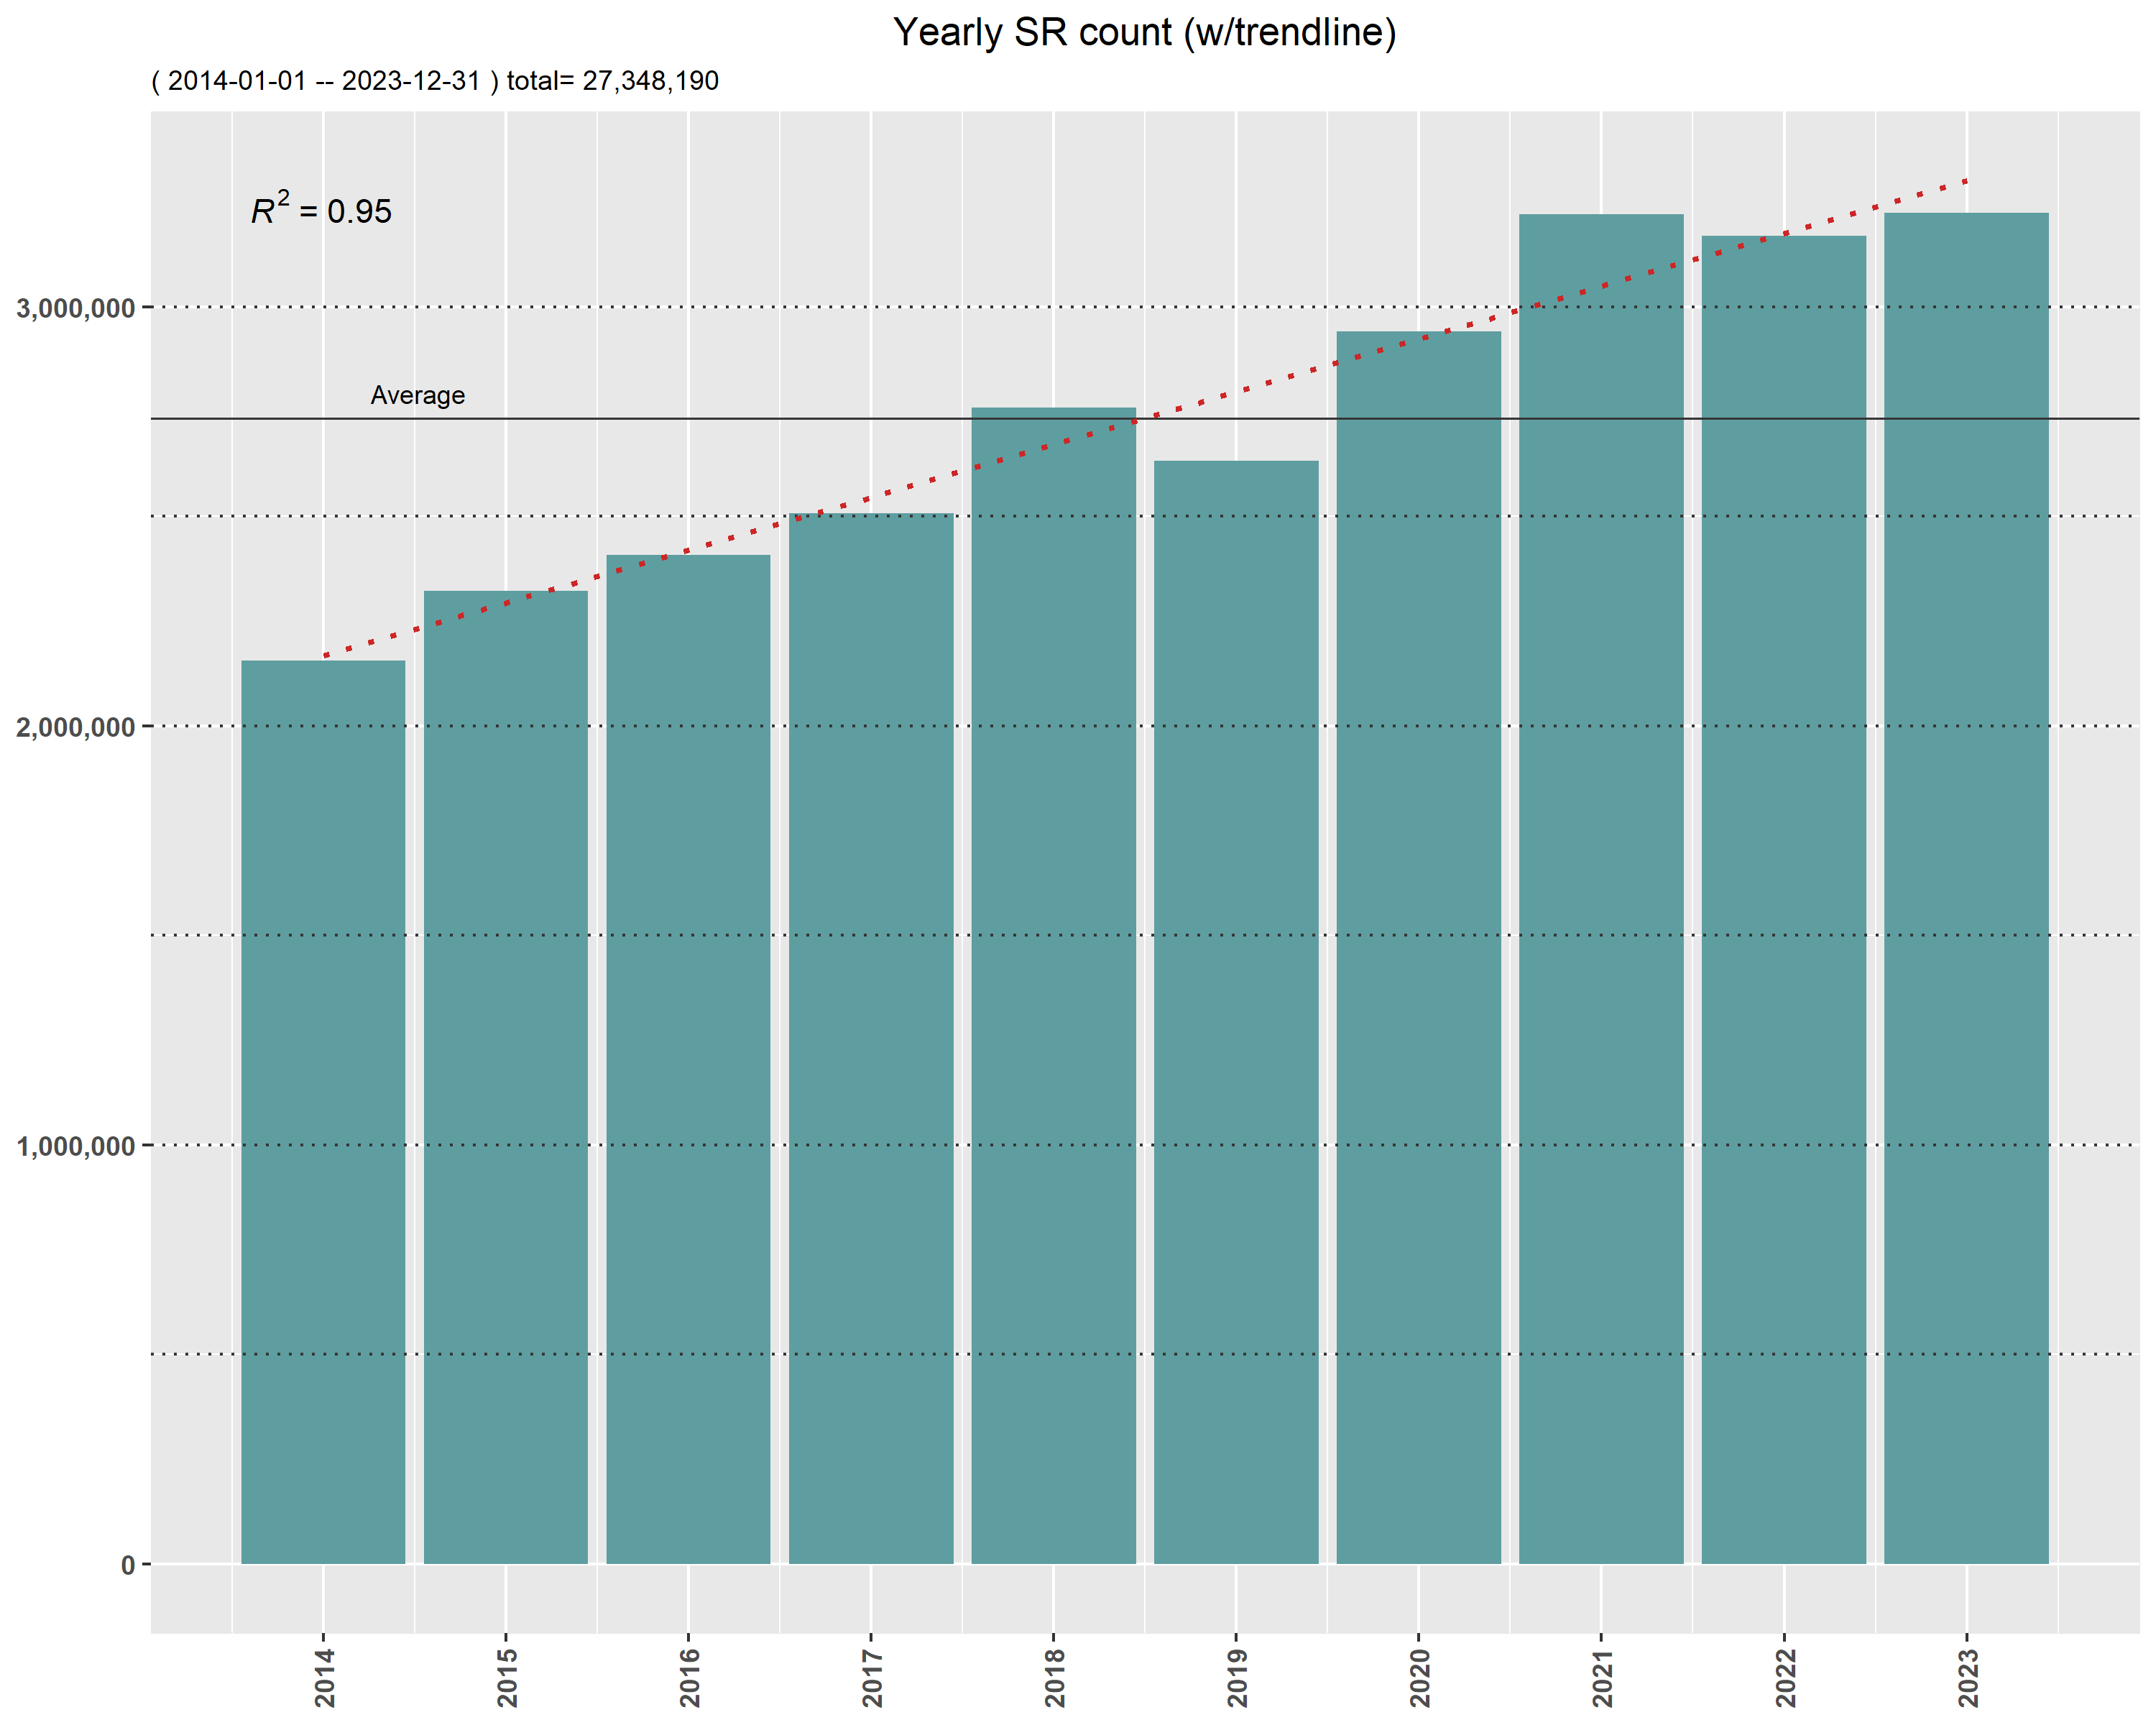
\includegraphics[width=\textwidth]{Yearly.png}
  \caption{SR counts by year for a 10-year period}
  \label{fig:yearly-counts}
\end{figure}

This 10-year timeframe (2014-2023) included the COVID pandemic impact. Note that the pandemic
impact reached a peak in the July-September 2020 timeframe, accompanied by additional spikes
in the 2\textsuperscript{nd}half of 2021 as well. The all-time daily high for SRs occurred on Tuesday, 2020-08-04, with a spike of
24,415 SRs, a full 9.8 \textsigma's from the mean. 

This below chart shows the 10-year period by calendar month. Note that almost all the months before the COVID pandemic outbreak in Feb/Mar
of 2020 are ``below average'', while most of the months after that period are ``above average'' months. And that trend of higher usage
of the 311 system has continued into the early months of 2024.

\begin{figure}[htbp]
  \centering
  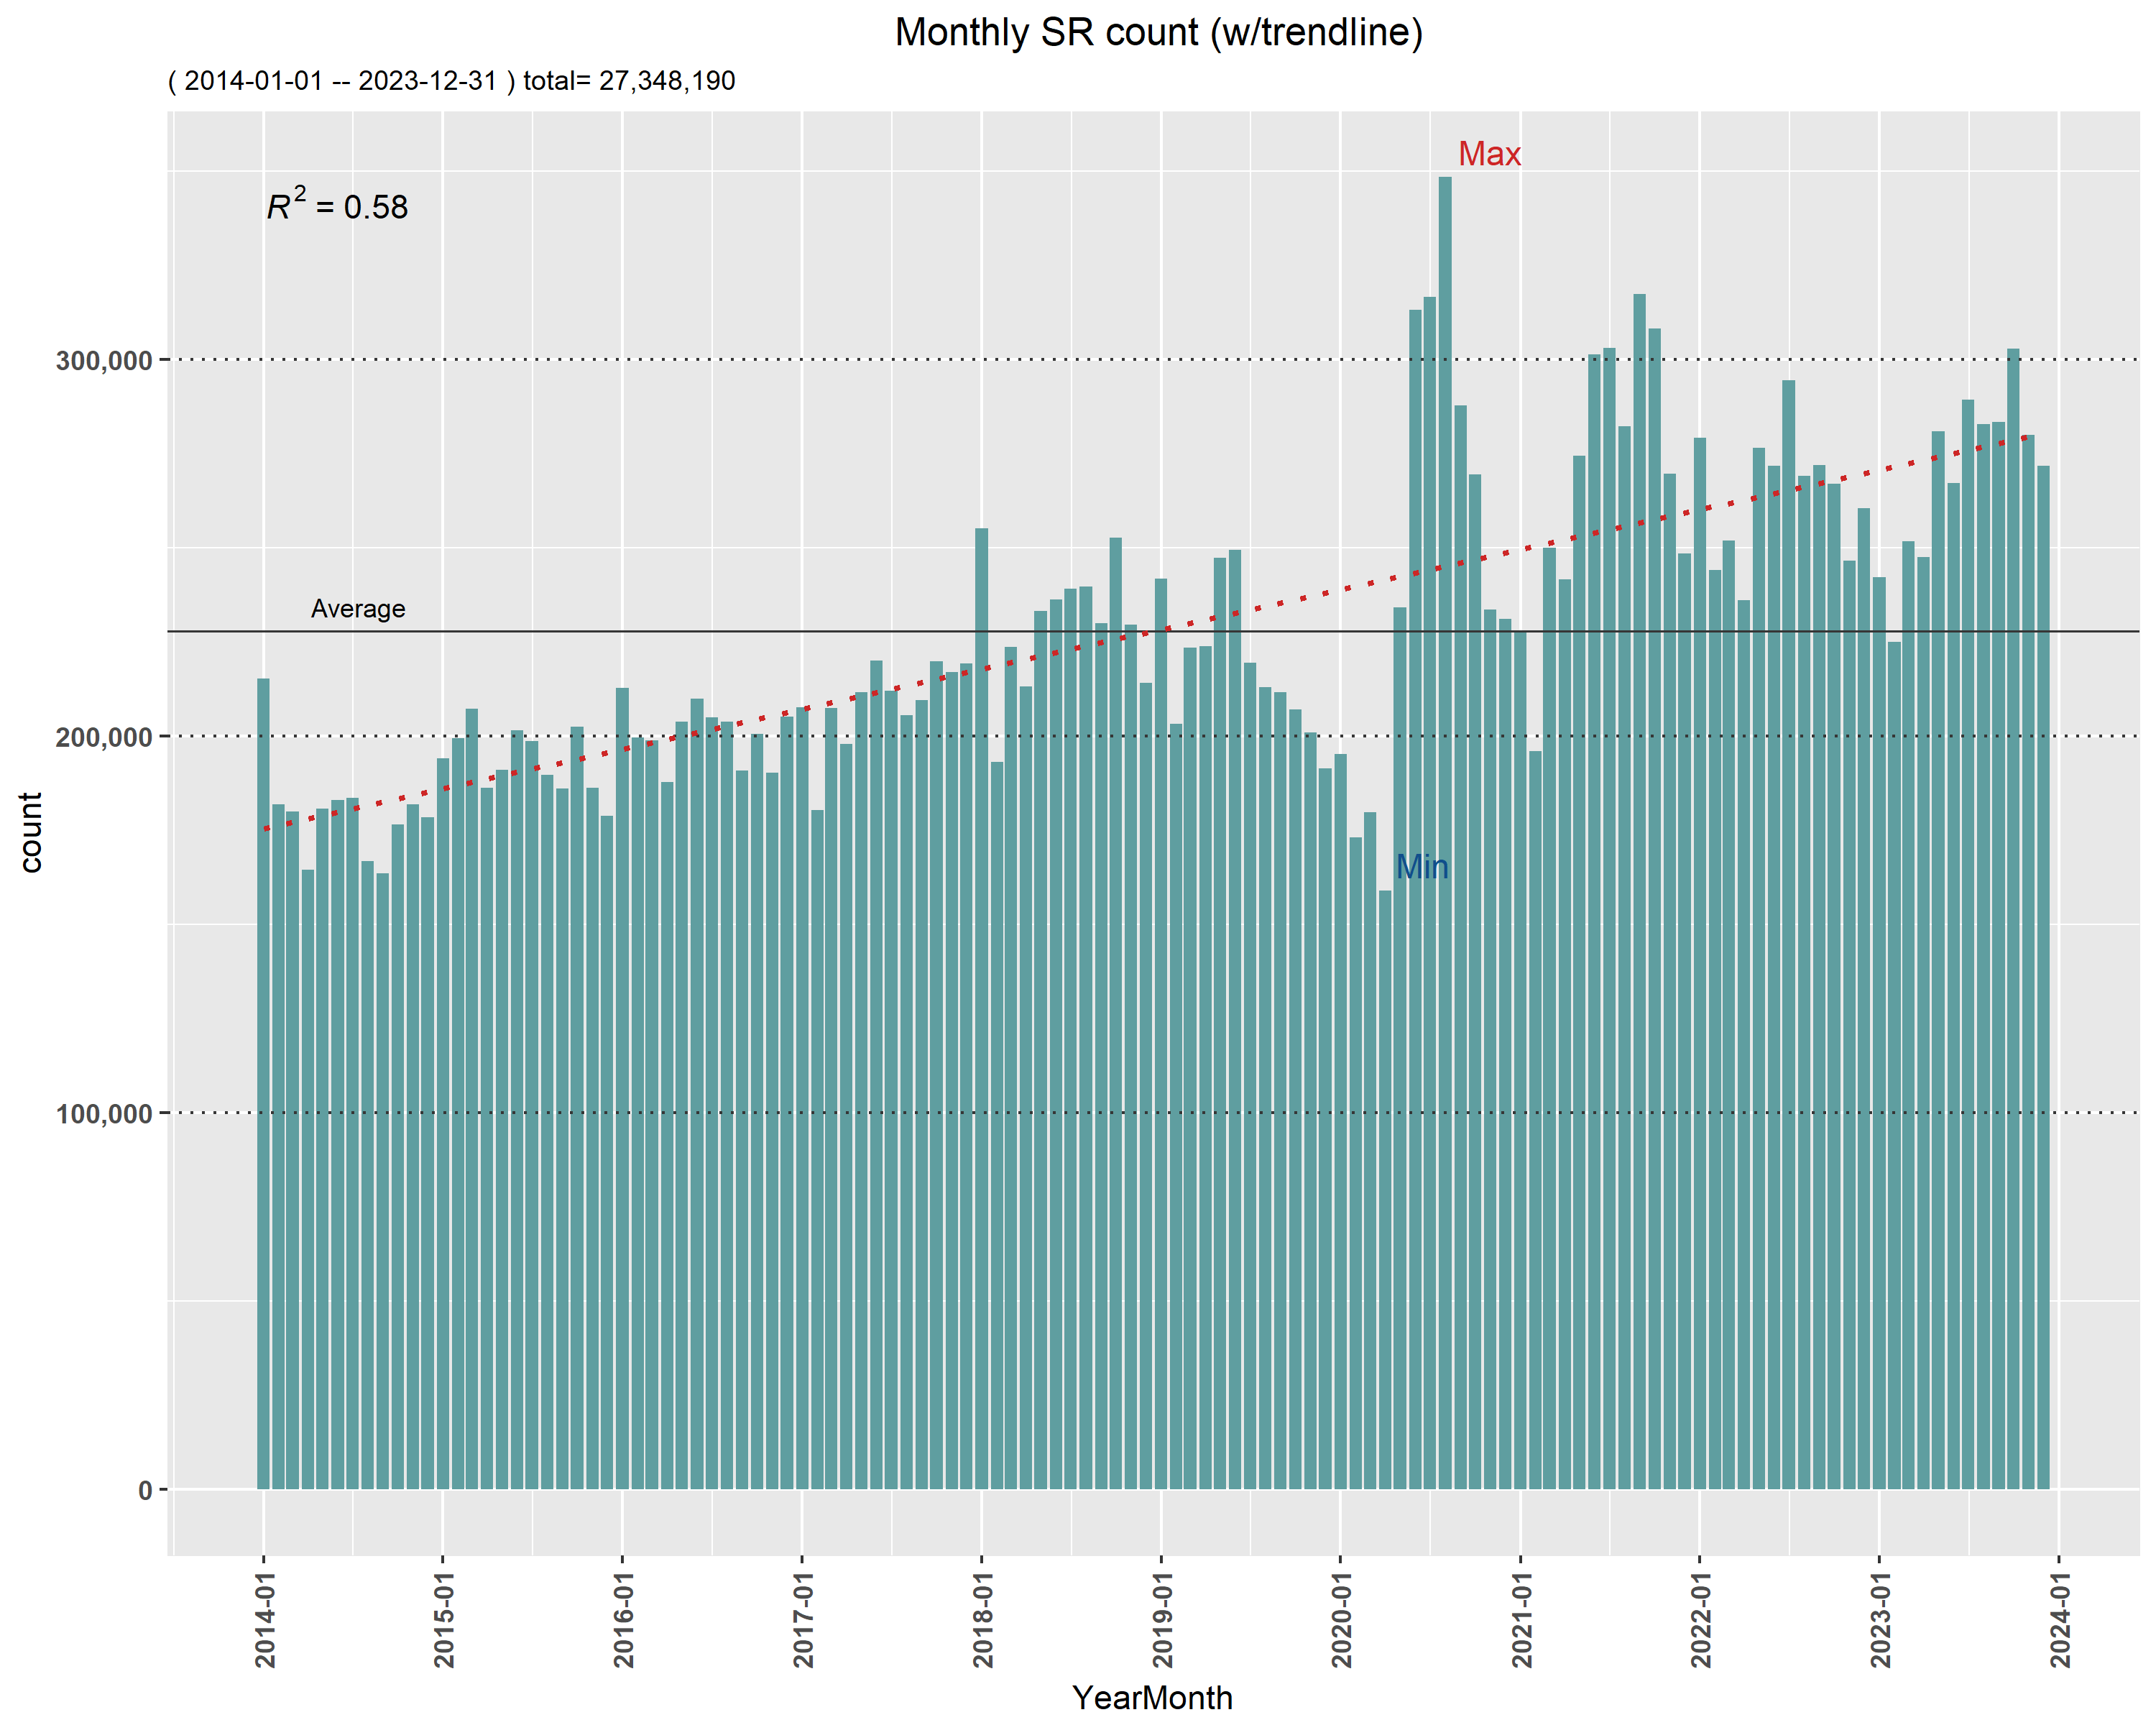
\includegraphics[width=\textwidth]{Monthly.png}
  \caption{SR counts by month for a 10-year period}
  \label{fig:monthly-counts}
\end{figure}

A quick look at the corresponding  daily tend over that same 10-year period is also interesting, as it shows both significant spikes
and significant dips; a noisy graph. While the spikes on 2020-08-04 (24,415 SRs) and 2020-08-05 (19,560 SRs) are COVID related, we are unable to 
ascertain any reason for the significant spike on Saturday, 2023-09-29 where 17,962 SRs were created.

\begin{figure}[H]
  \centering
  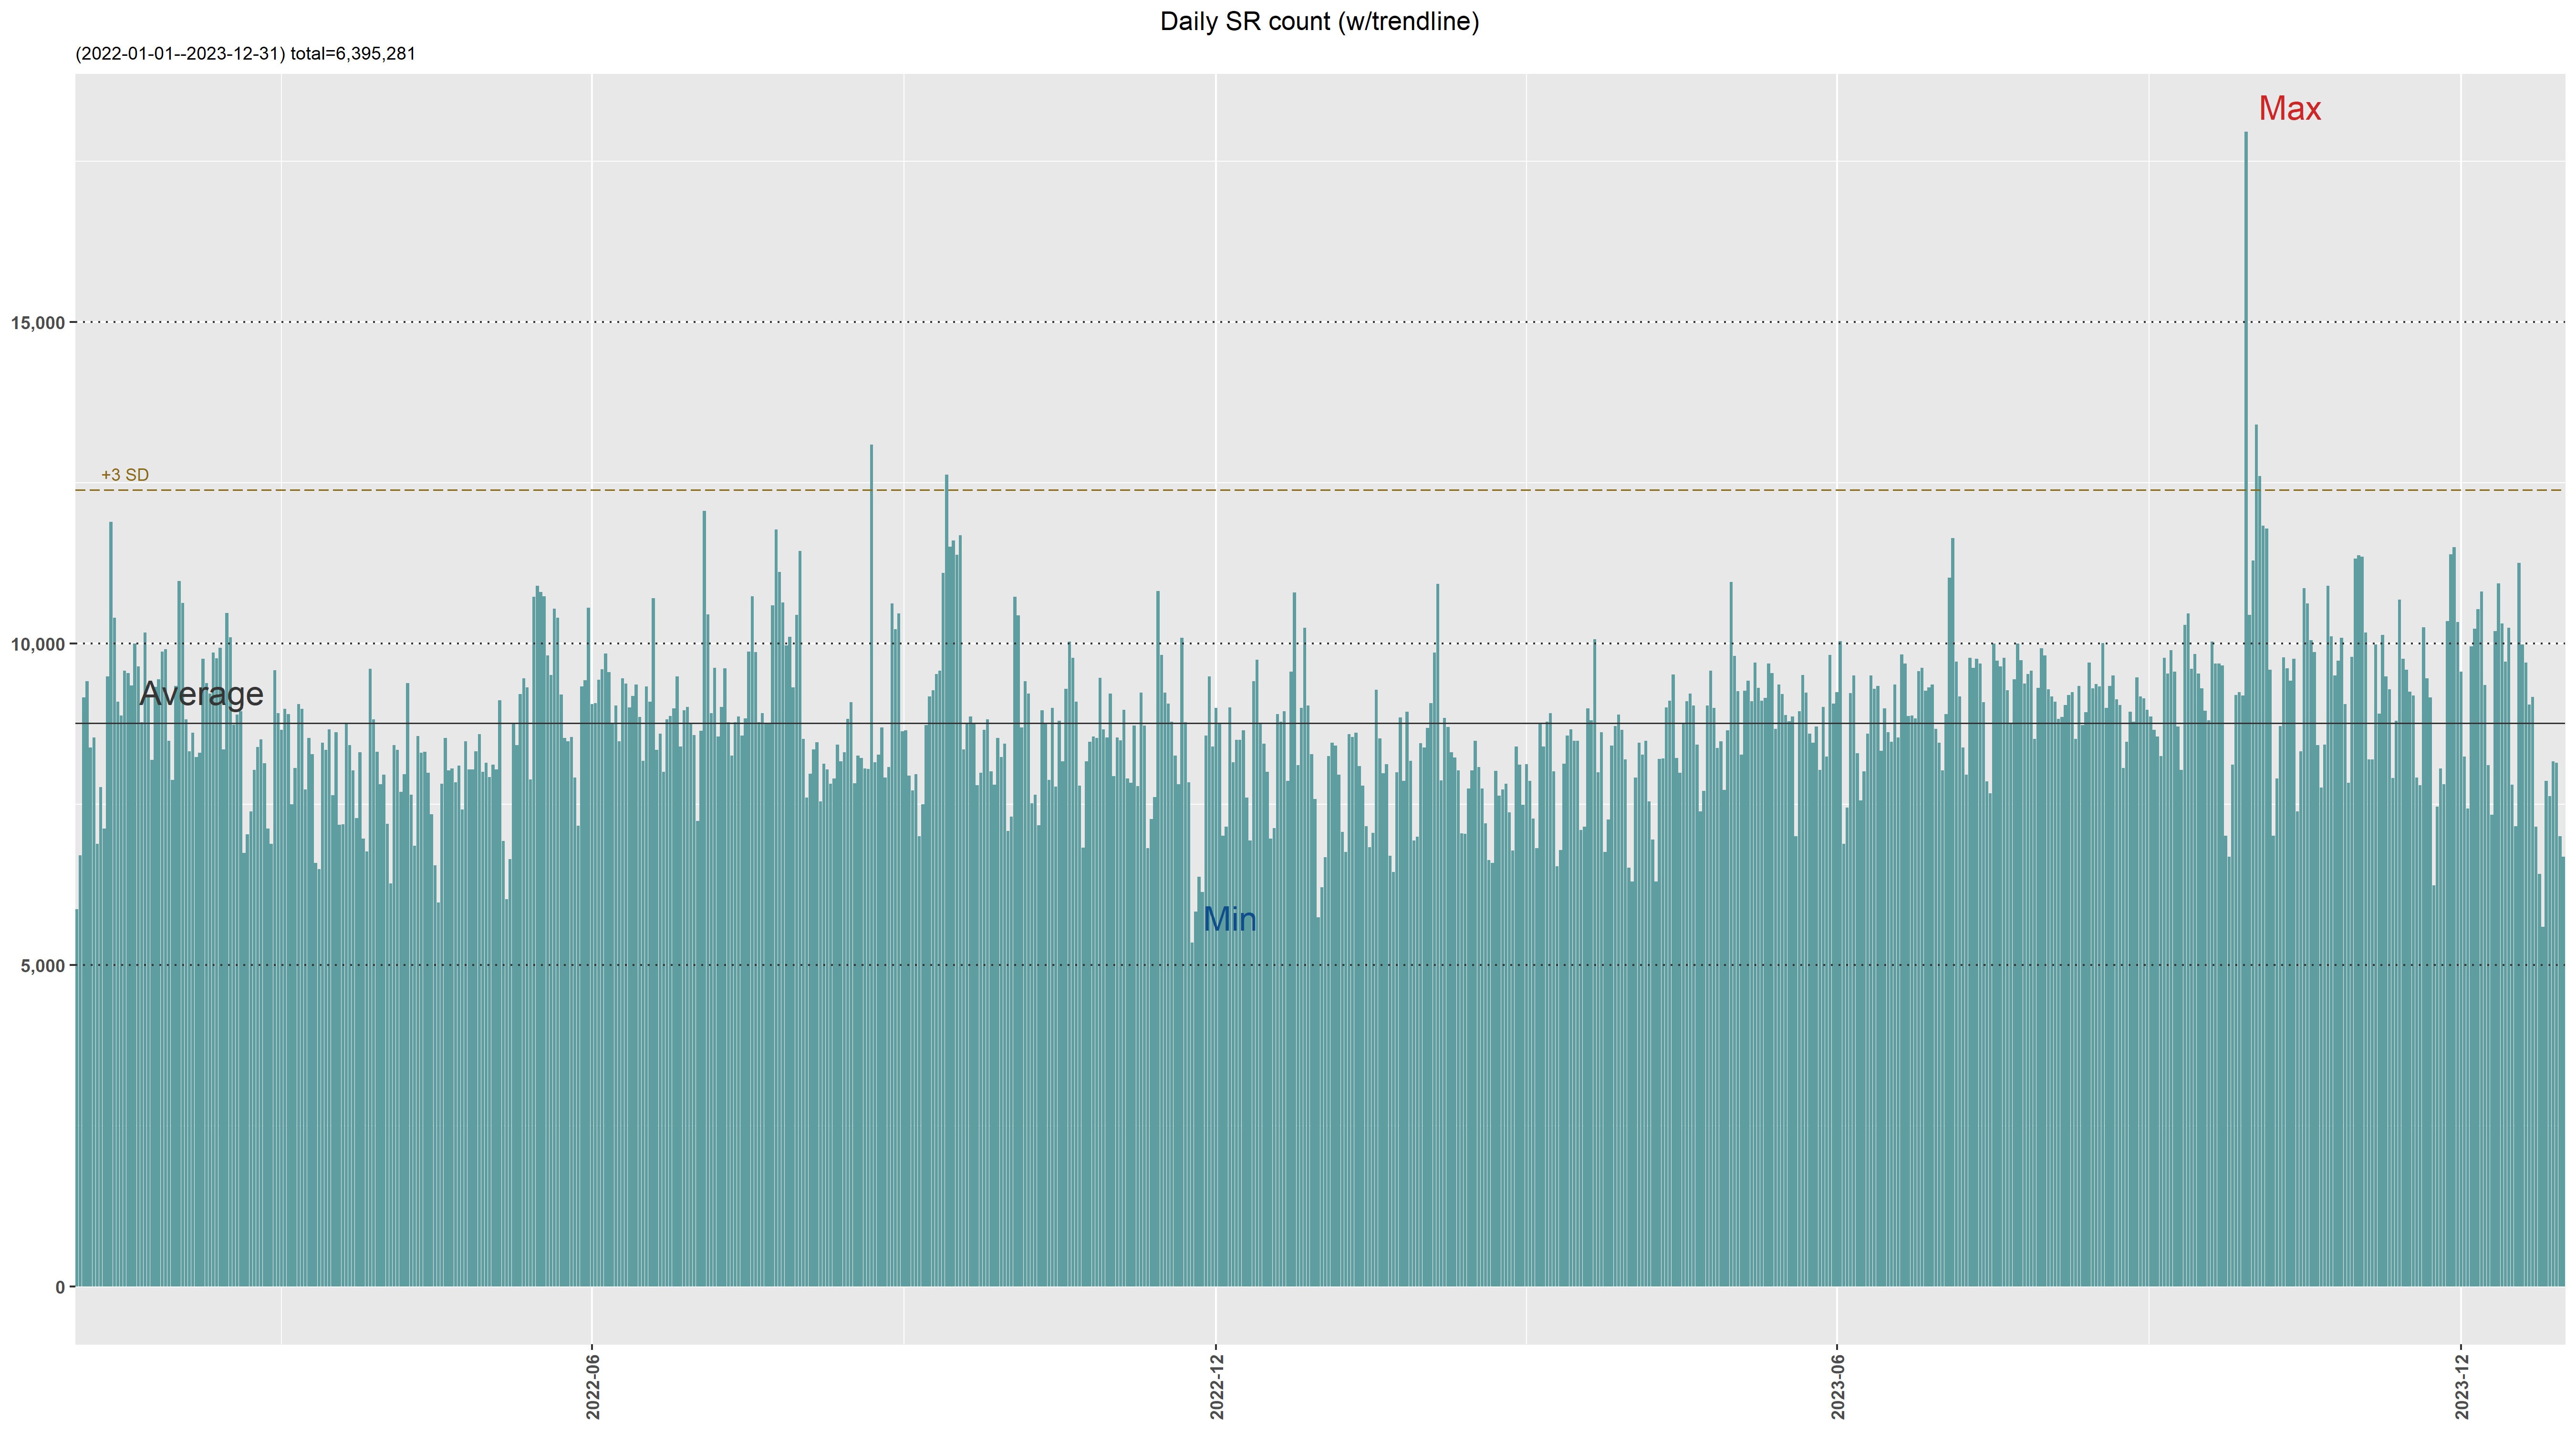
\includegraphics[width=\textwidth]{Daily.png}
  \caption{SR counts by day for a 10-year period}
  \label{fig:daily-counts}
\end{figure}

Seasonal trends are also prevalent. The months of November-thru-April are ``below average'' months, while the months May-thru-October are ``above average''. 
This seasonal trend is observed throughout the 10-year period.

\begin{figure}[H]
  \centering
  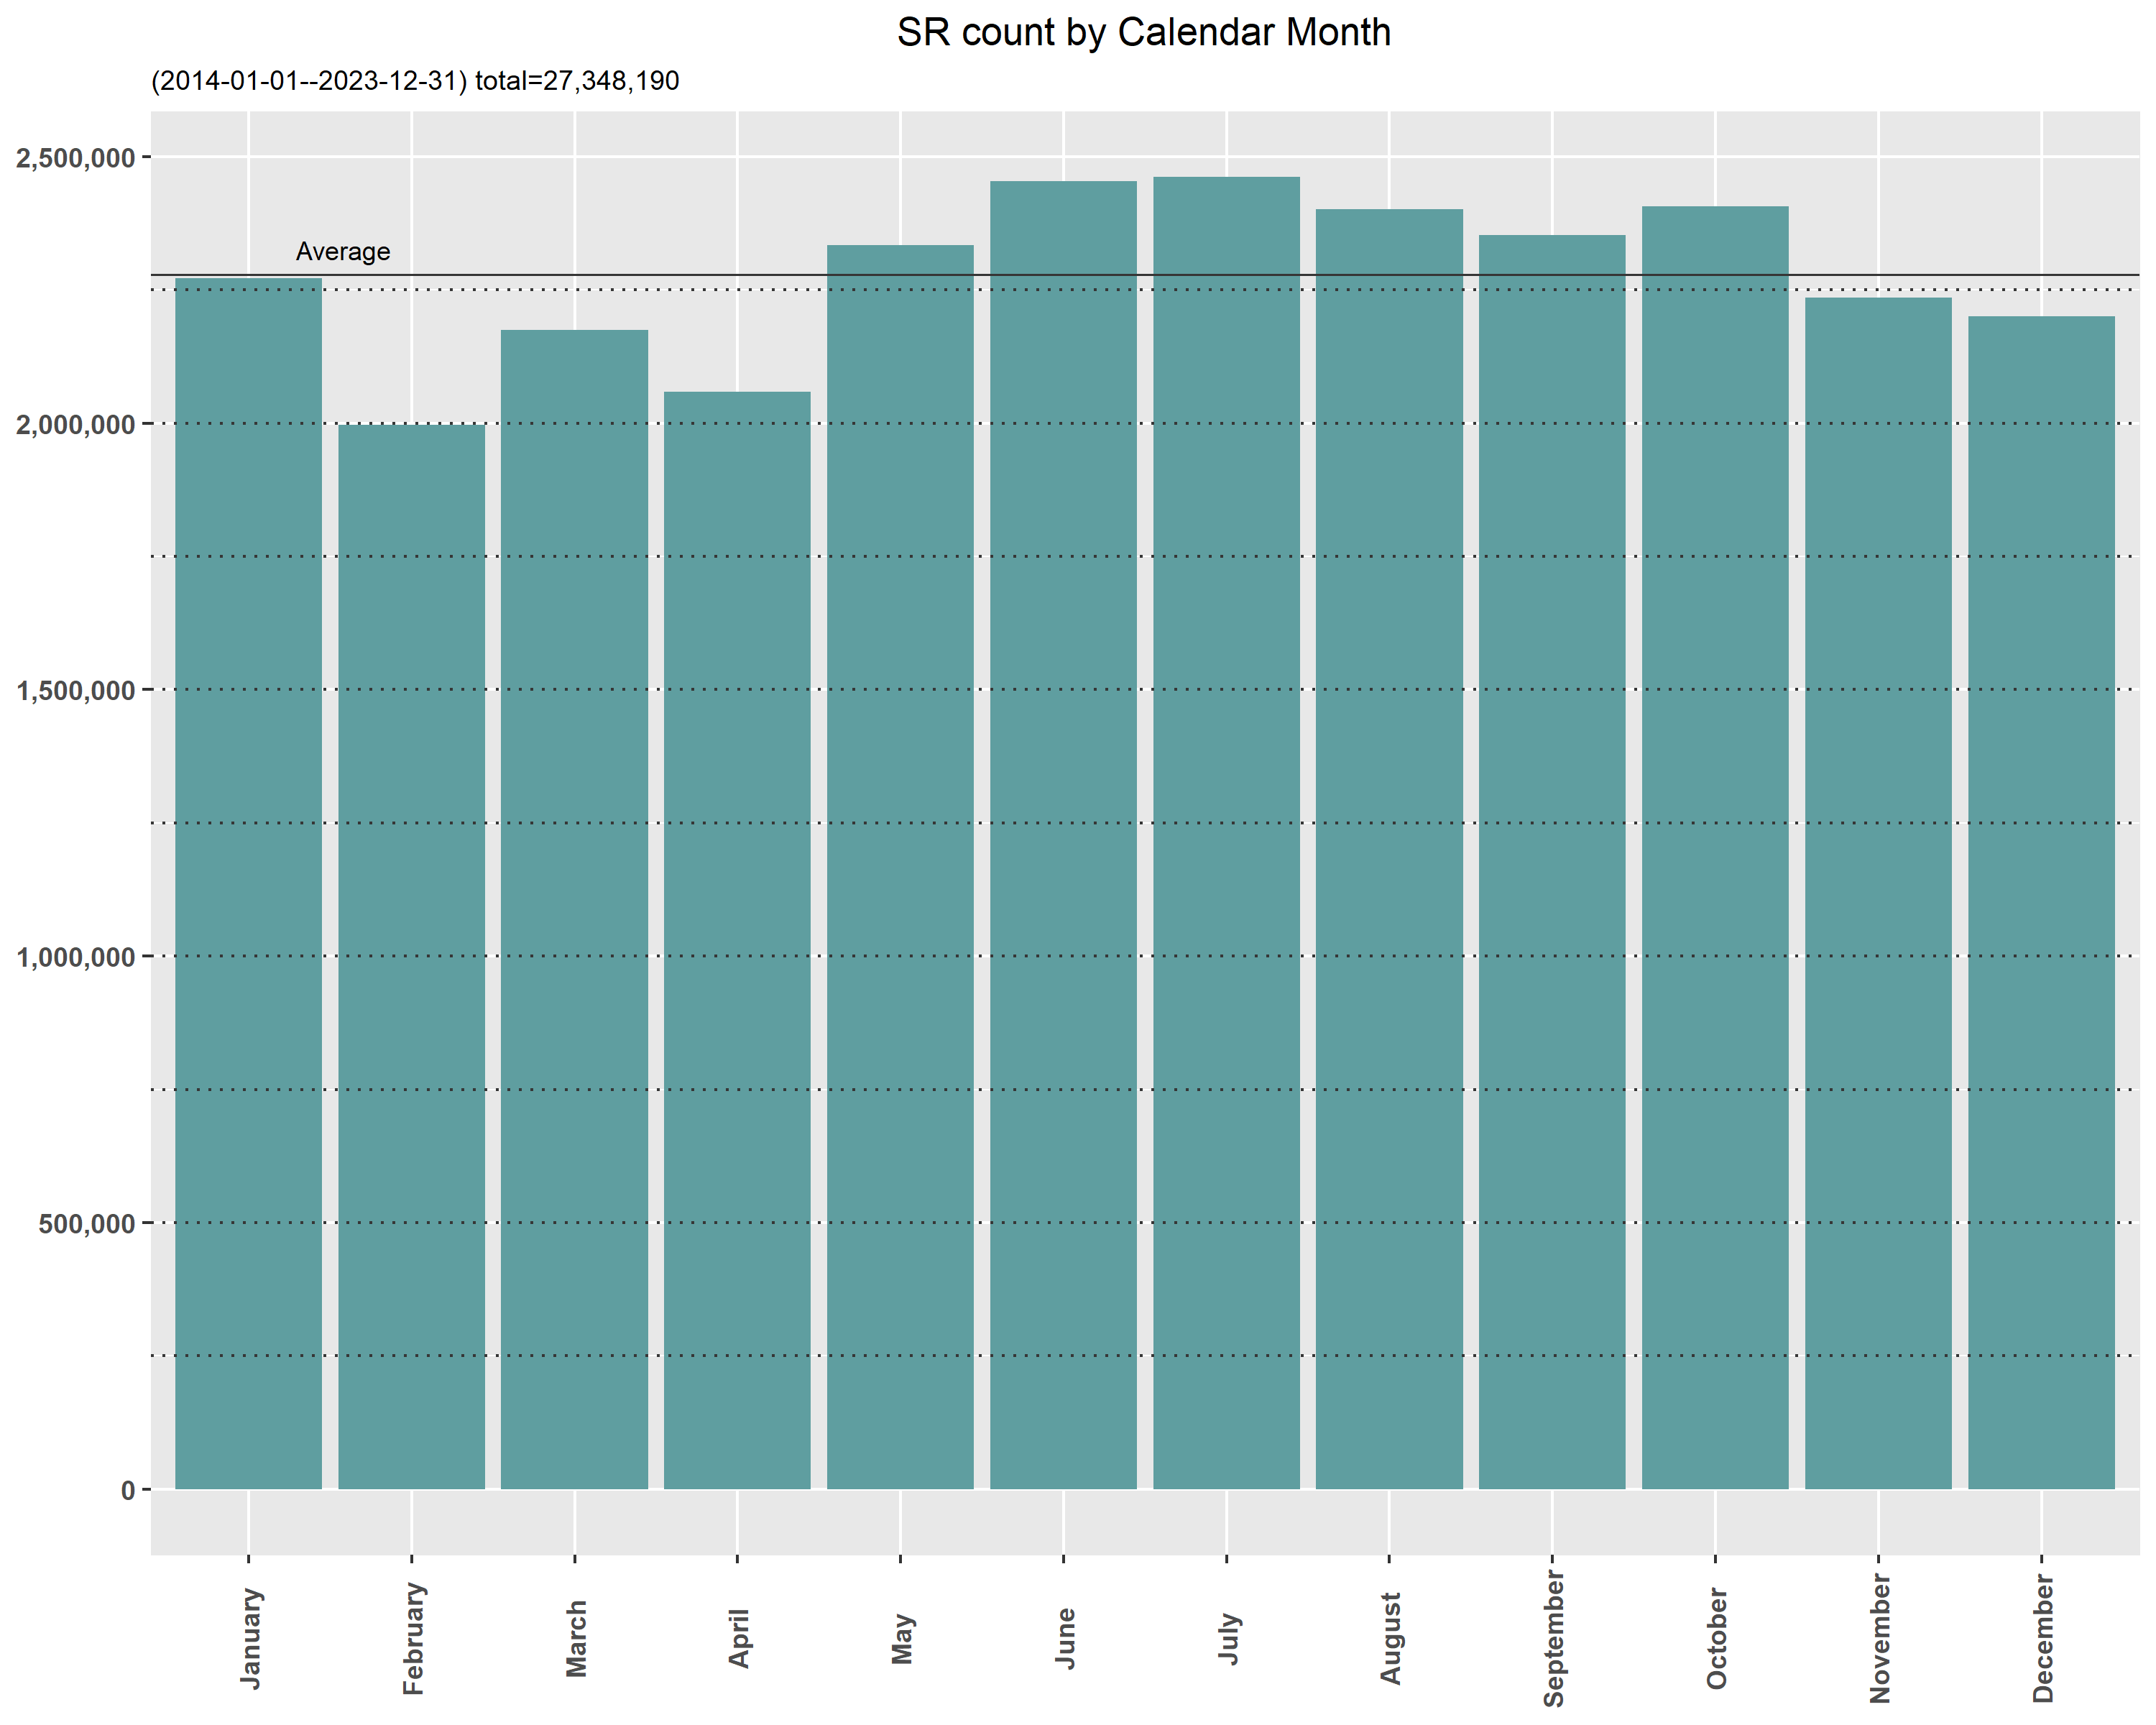
\includegraphics[width=\textwidth]{Calendar-Month.png}
  \caption{SR counts by calendar month for a 10-year period}
  \label{fig:calendar-months-counts}
\end{figure}

Of note, the lowest SR counts-per-day occur on Christmas  period (+/- a day), in 5 of the Bottom 10 SR counts-per-day. The summer moths and early
fall months make up all of the Top 10 SR counts-per-day. As previously noted, the all-time daily high for SRs occurred on Tuesday, 2020-08-04 with the 10-year
low number occurs on Christmas Day in 2016, a Sunday. Note also that the difference between the peak day (24,415) and the minimum day (2965) varies
by a factor of 8X, and the aveage daily count of 7489 -- all of which creates a challenging  system capacity design issue.

\begin{table}[htbp]
	\begin{minipage}[t]{0.35\textwidth} % Adjust the width of the minipage as needed
	\centering
	\small % Adjust the font size
	\caption{Top 10 days}
	\label{tab:top_ten_counts}
		\begin{tabular}{@{}lll@{}}
			\toprule
			Date & Count & Rank \\
			\midrule
			2020-08-04 & 24415 & 1 \\
			2020-08-05 & 19560 & 2 \\
			2023-09-29 & 17962 & 3 \\
			2020-07-05 & 16916 & 4 \\
			2020-06-21 & 15883 & 5 \\
			2020-06-20 & 15825 & 6 \\
			2020-07-04 & 15794 & 7 \\
			2021-09-02 & 15205 & 8 \\
			2020-06-28 & 14057 & 9 \\
			2021-10-28 & 13575 & 10 \\
			\bottomrule
		\end{tabular}
	\end{minipage}\hfill % Adjust the space between the tables
	\begin{minipage}[t]{0.35\textwidth} % Adjust the width of the minipage as needed
	\centering
	\small % Adjust the font size
	\caption{Bottom 10 days}
	\label{tab:bottom_ten_counts}
		\begin{tabular}{@{}lll@{}}
			\toprule
			Date & Count & Rank \\
			\midrule
			2014-12-25 & 2965 & 1 \\
			2015-12-25 & 3247 & 2 \\
			2014-04-20 & 3287 & 3 \\
			2015-12-26 & 3405 & 4 \\
			2016-11-06 & 3419 & 5 \\
			2014-07-04 & 3455 & 6 \\
			2014-12-27 & 3534 & 7 \\
			2014-09-14 & 3563 & 8 \\
			2014-02-02 & 3565 & 9 \\
			2016-12-25 & 3587 & 10 \\
			\bottomrule\\
		\end{tabular}
	\end{minipage}
\end{table}

And although the highest number of SRs occur in July and the lowest in February,
when the \#-of-SRs-per-day metric is computed by adjusting for the differing number of days for each month -- the
busiest month is shown to be June (followed by July and September). And similarly the quietest months are April, March, and 
February. In general, the winter months see fewer SRs while the summer months show 
an increase in activity, as previously noted.

\begin{table}[ht]
    \centering
    \small
    \begin{tabular}{lS[table-format=7.0]S[table-format=6.0]} % 'l' for left-aligned, 'S' for siunitx number alignment
        \toprule
        \textbf{Month}     & \textbf{Count}   & \textbf{Count per Day} \\ 
        \midrule
        June  & 2454156 & 81805 \\ 
        July  & 2461525 & 79404 \\ 
        September & 2352822 & 78427 \\ 
        October & 2407238 & 77653 \\ 
        August & 2401731 & 77475 \\ 
        May  & 2334466 & 75305 \\ 
        November  & 2236037 & 74535 \\ 
        January   & 2271524 & 73275 \\ 
        December  & 2199765 & 70960 \\ 
        February  & 1996408 & 70795 \\ 
        March & 2174349 & 70140 \\ 
        April  & 2058169 & 68606 \\ 
       \bottomrule
    \end{tabular}
    \caption{Monthly counts sorted by counts-per-day}
    \label{tab:monthly_counts}
\end{table}

\FloatBarrier % Ensure all floats before this point are processed before moving on

Two areas that are important in this data cleansing analysis effort are the responsible NYC Agency, and the actual type of complaint.
Given both the size of the City of New York government, it's typically necessary to identify the responsible Agency as well as the type of complaint in order to 
clarify the responsible area and assist in troubleshooting any discrepancy.

In discovering a data error, we typically observe two trends; either a single (or a small few) Agencies are responsible (such as Dept of Transportation), or it is a system-wide issue that foolows the general distribution
of  Service Requests (SRs) across the system. Let's take a brief look at how this plays out across the system, so when we identify a
issue, it will be useful to see how that issue flows back to a specific Agency, and thus establish responsibility.

Although the 311 SRs involve 16 different agencies, there are the ``big six'' Agencies that comprise
90\% of the complaints. These six are (in order):  

\begin{itemize}
	\item New York Police Department (NYPD)
	\item Housing Preservation \& Development (HPD
	\item New York City Department of Sanitation (DSNY)
	\item Department of Transportation (DOT)
	\item Department of Environmental Protection (DEP)
	\item Department of Parks \& Recreation (DPR)
\end{itemize}

\begin{figure}[htbp]
  \centering
	  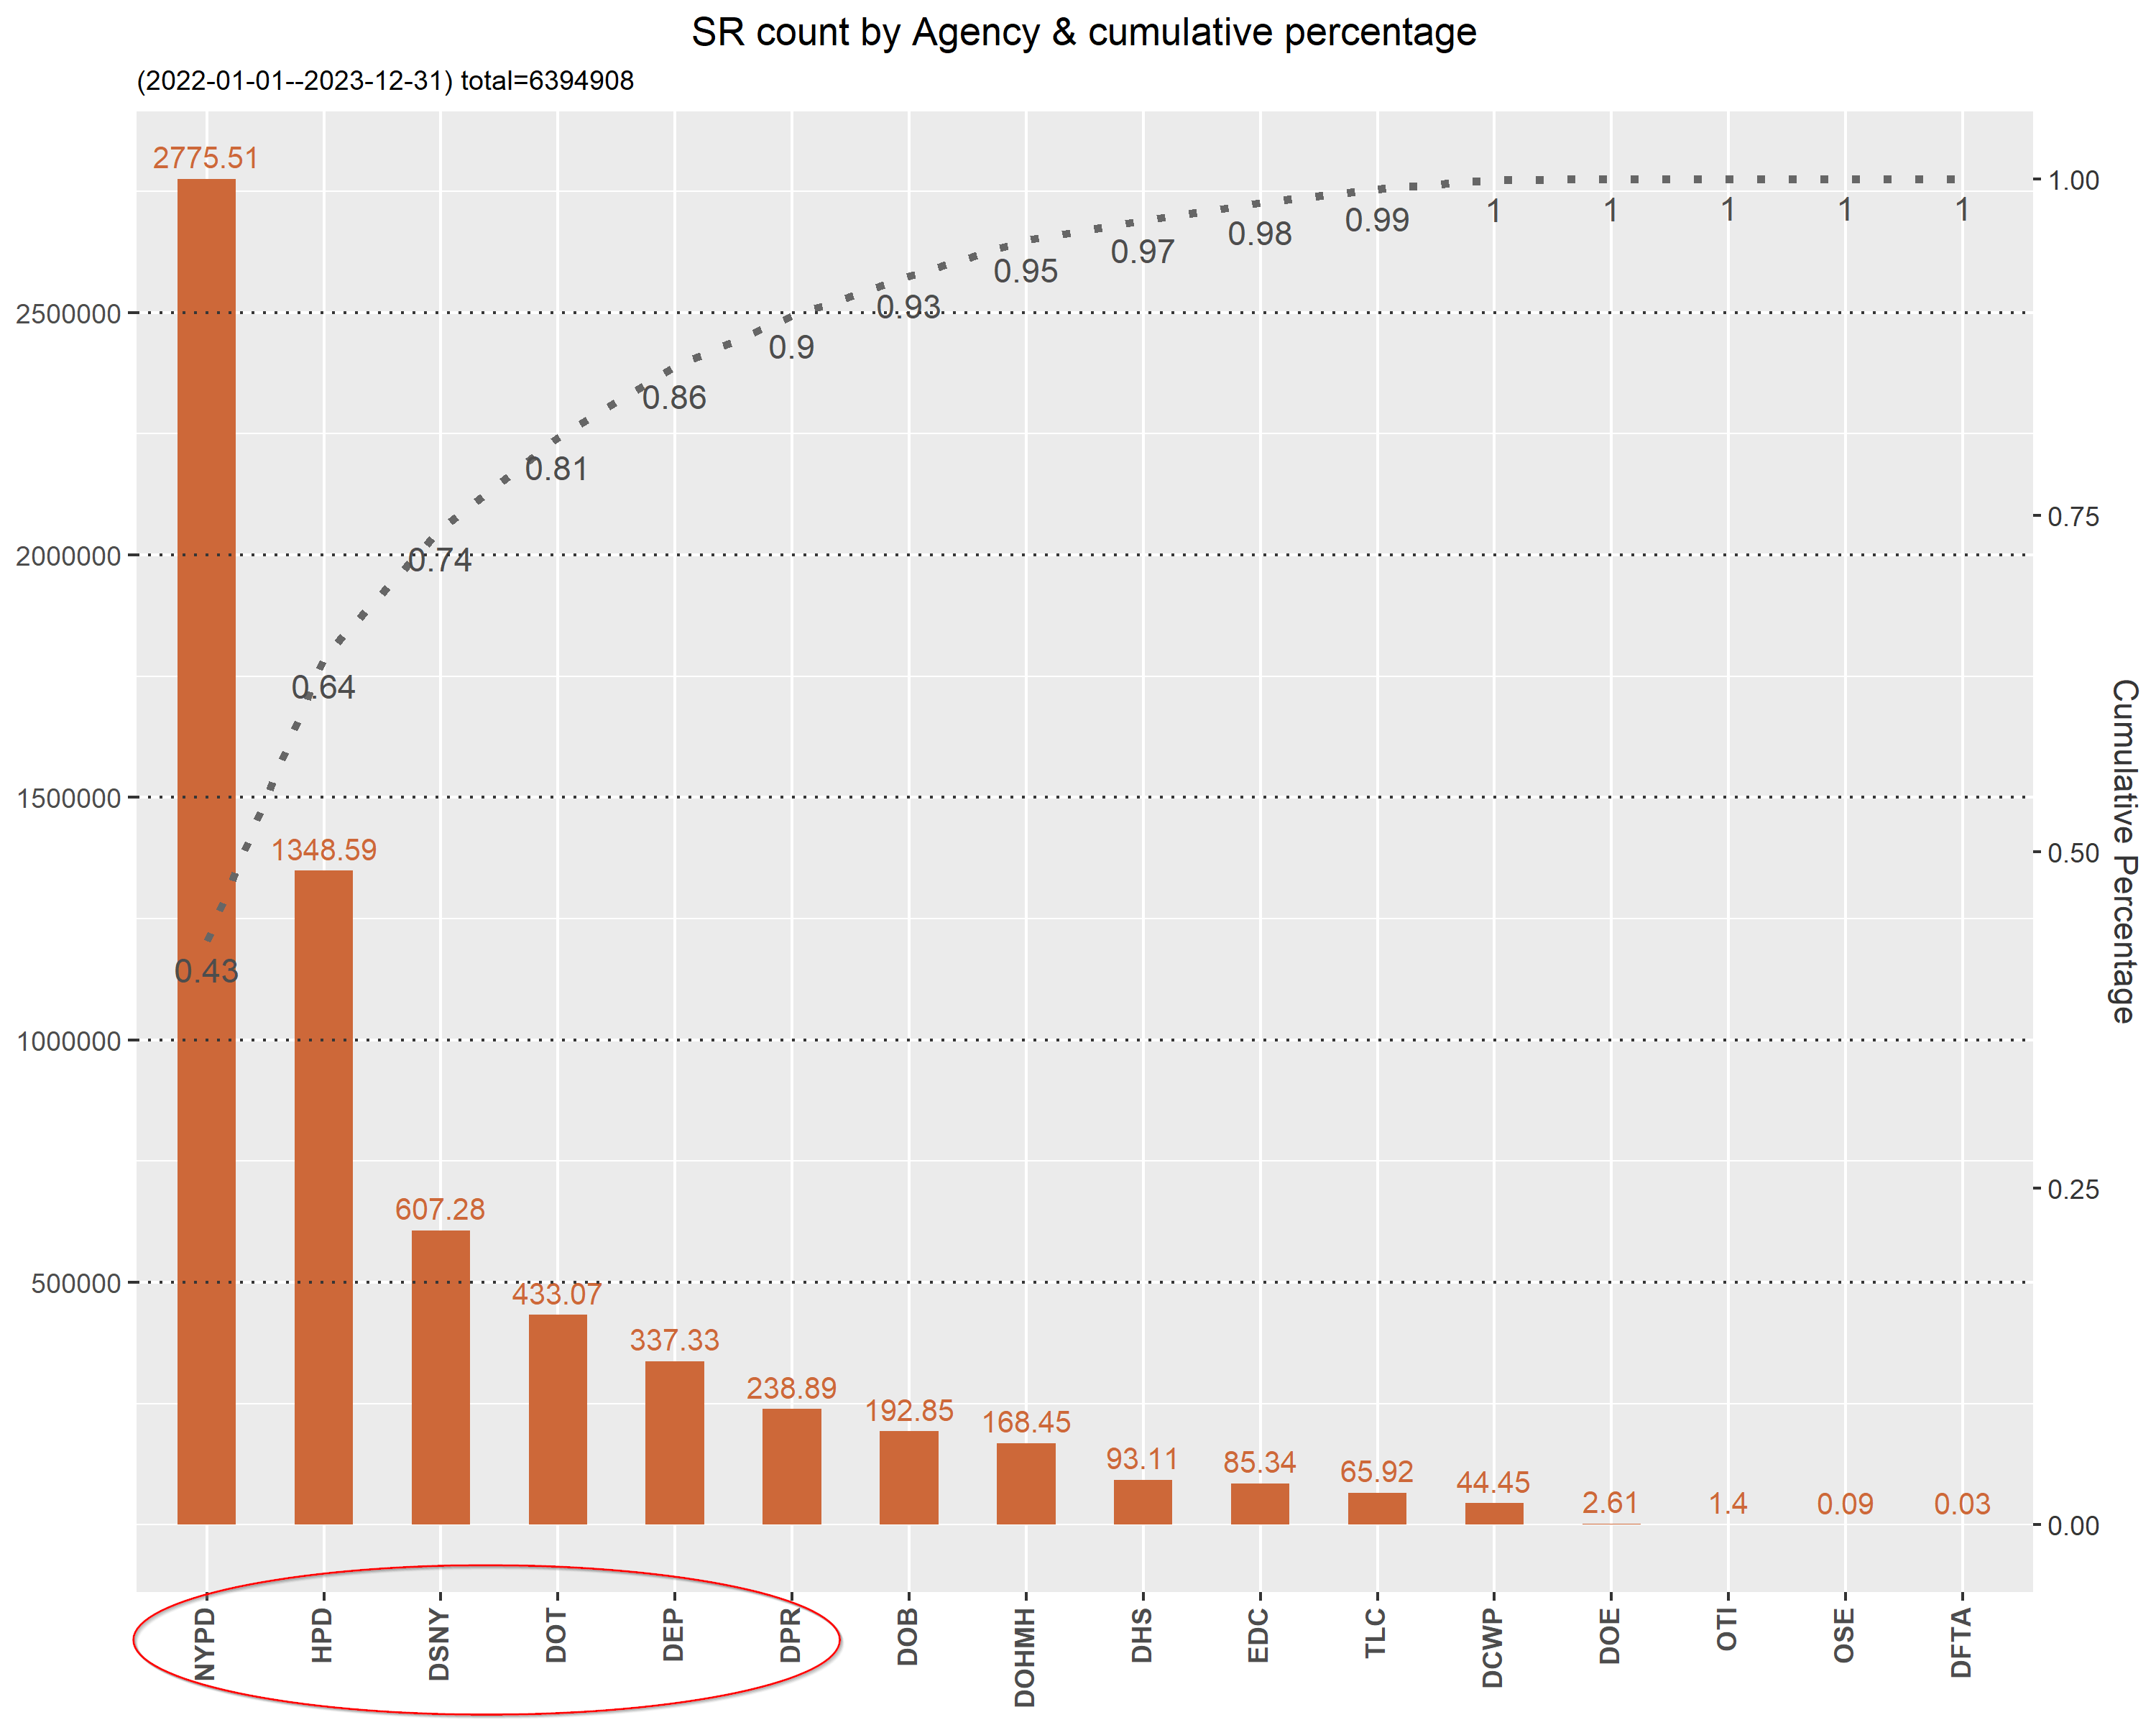
\includegraphics[width=\textwidth]{SRs_by_Agency.png}
	  \caption{SR counts by Agency and Cumulative Percentage}
	  \label{fig:SR_counts_by_Agency}
\end{figure}

It is also interesting to note the distribution of the type of complaints in the 311 SR dataset; it is heavily skewed to  a select few complaints.

\begin{figure}[htbp]
  \centering
	  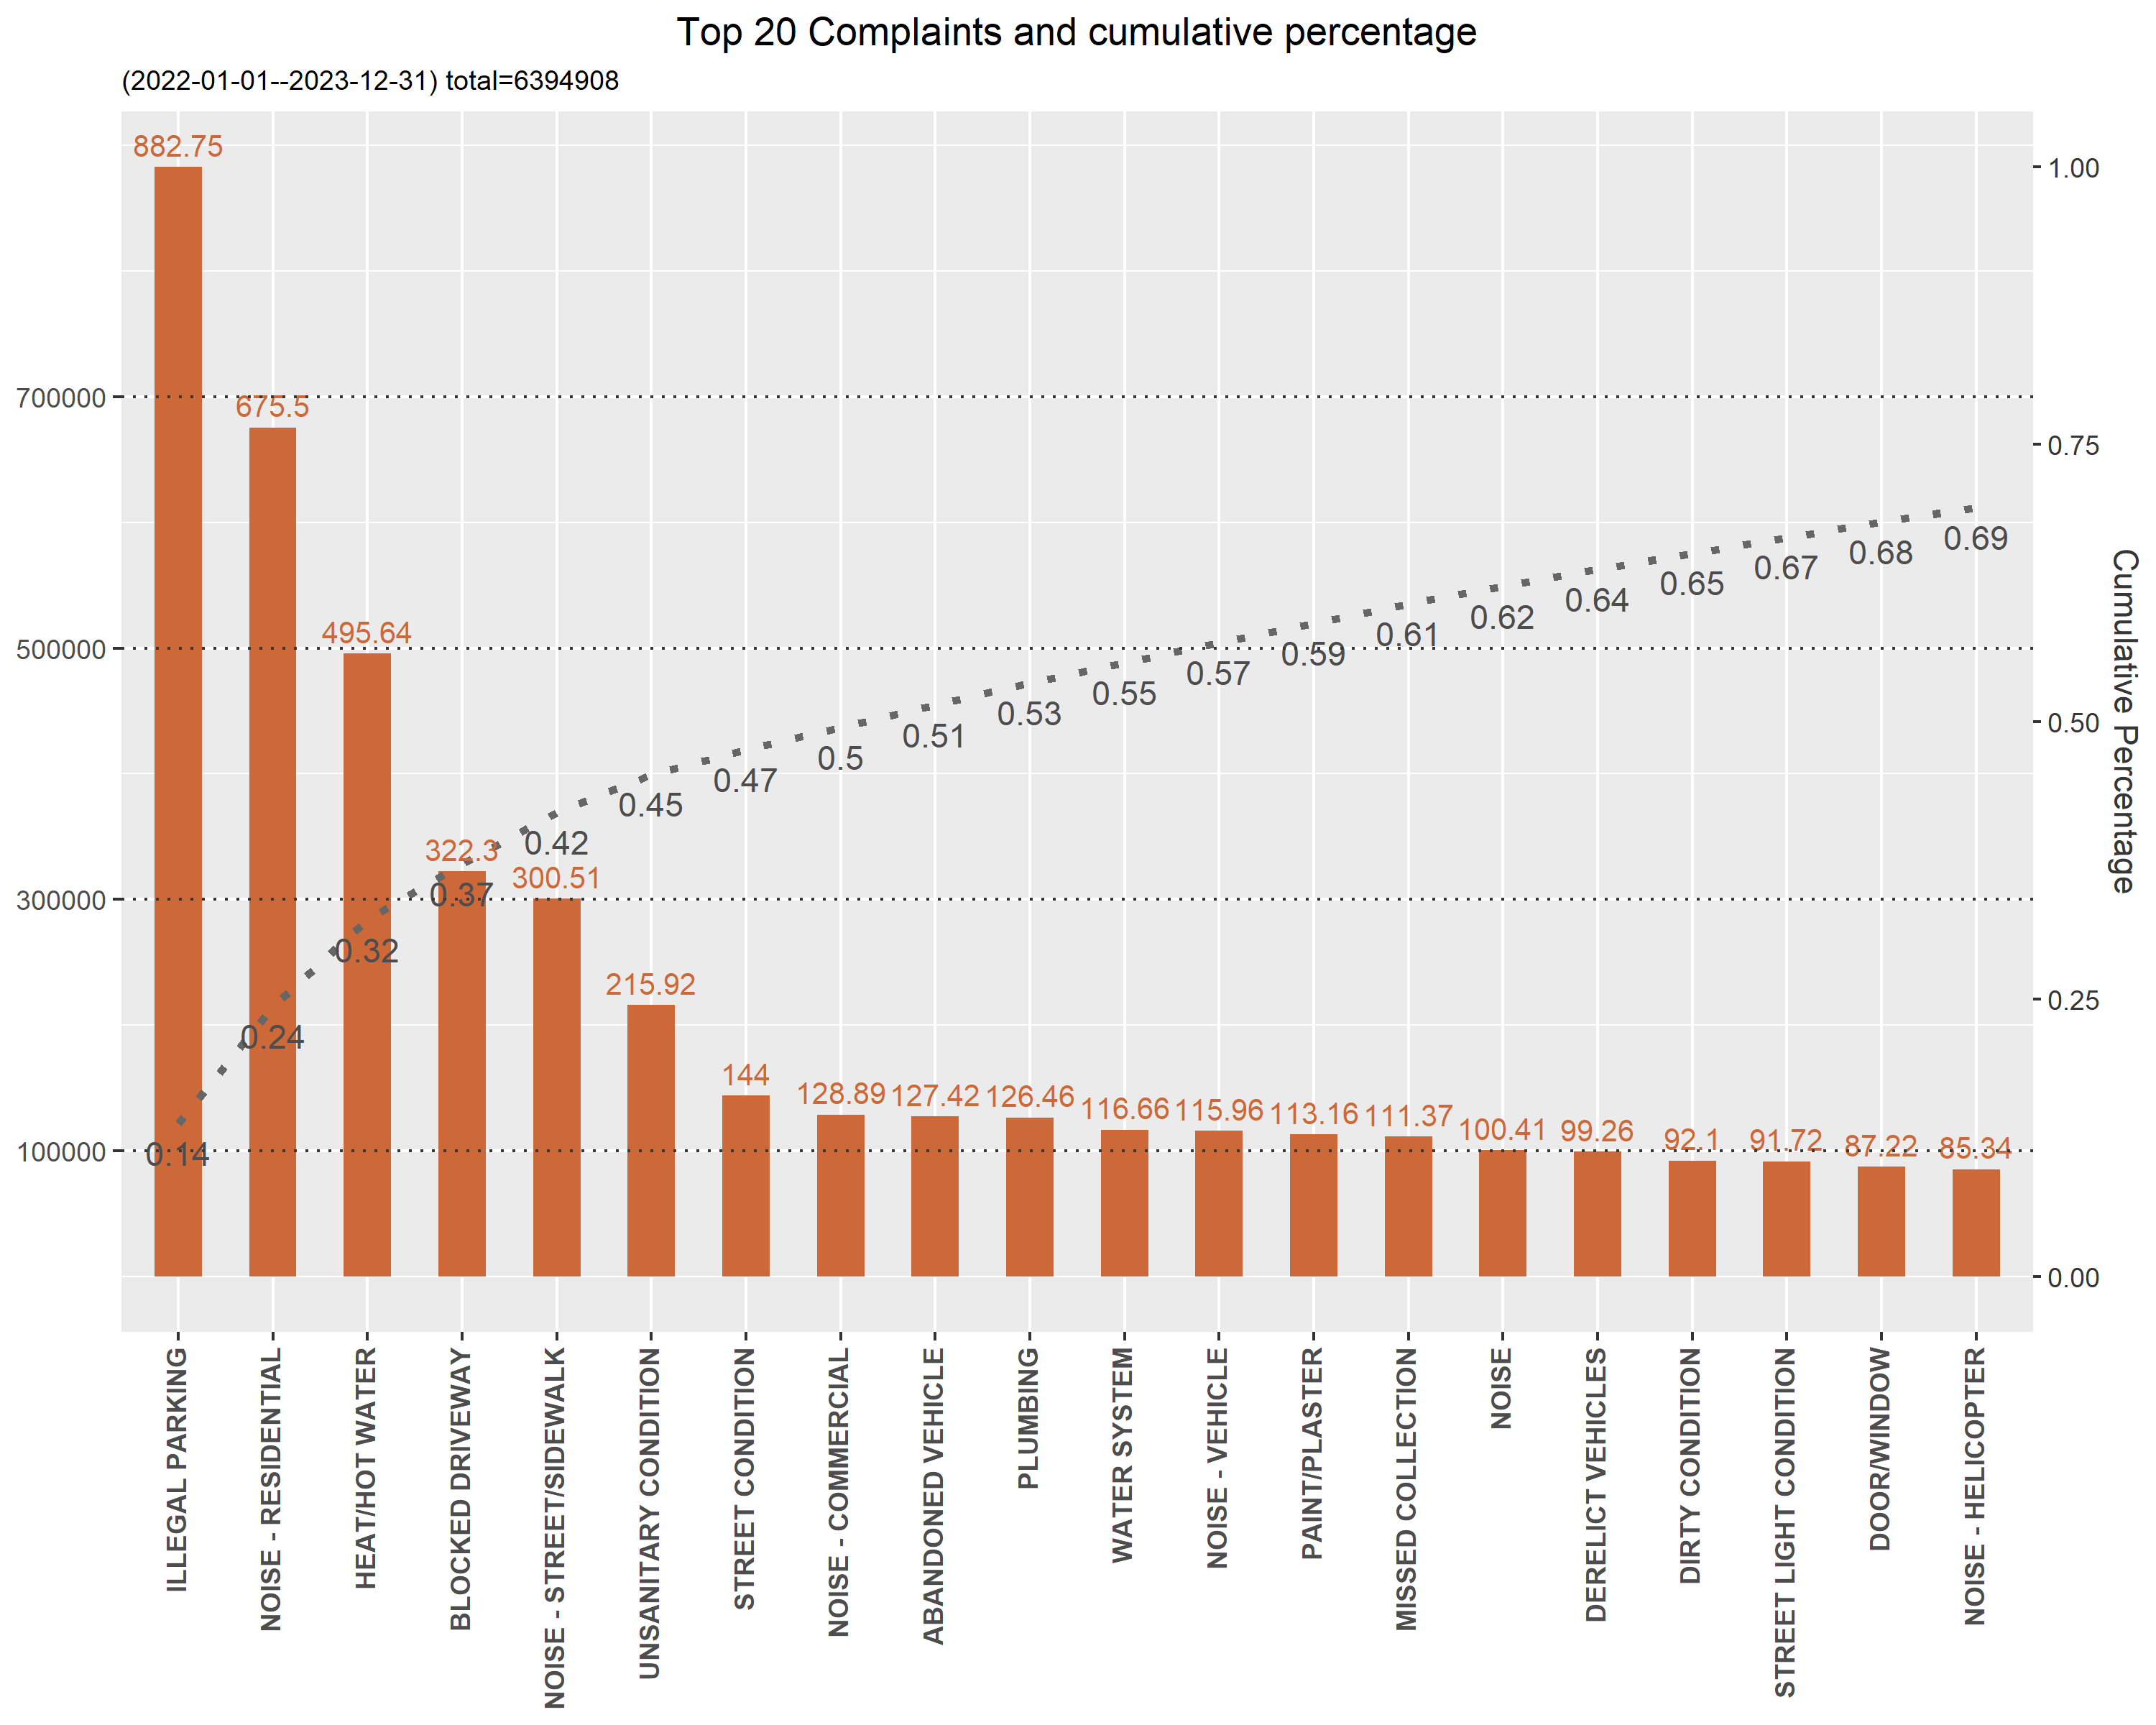
\includegraphics[width=\textwidth]{SRs_by_Complaint_Type.png}
	  \caption{Top 20 SR Complaints and Cumulative Percentage}
	  \label{fig:SR_complaints}
\end{figure}

The top 20 complaints contain several of the eight different types of ``Noise'' complaints (Residential, Commercial, Street, Helicopter, etc.). These Noise-related
complaints total 1.435 million in the 2022-2023 dataset, a full 22\% of all complaint types, which is the most frequently occurring type. (Note: Ilegal Parking is 
second, followed by Heat/Hot Water.) Noise complaints are also handled by NYPD, as is Illegal Parking and Blocked Driveway complaints, which mostly
accounts for the top ranking of 311 SRs being routed to the NYPD.

There are also some rather curious and unusual Service Requests in the 311 data: 
tanning, tattooing, trans fat, unsanitary pigeon condition, illegal animal kept as pet, harboring bees/wasps, and radioactive material. 
New Yorkers certainly live interesting lives. 

The NYC HPD handles about 49\% of what NYPD handles. For  non-NYC readers, 
HPD is the City agency that manages the  177,569 NYC public housing units as well as monitoring all rental and leased apartment units. HPD collectively
serves 528,105 people, a population larger than Atlanta or Miami. Hence the large number of Heat/Hot Water and Unsanitary complaints. 


\section{Potential Issues} \label{sec:issues}

What is data cleansing?  Wikipedia \href{https://en.wikipedia.org/wiki/Data_cleansing}{Data Cleansing} offers a good definition. 

``Data cleansing or data cleaning is the process of detecting and correcting (or removing) corrupt or inaccurate records from a record set, 
table, or database and refers to identifying incomplete, incorrect, inaccurate or irrelevant parts of the data 
and then replacing, modifying, or deleting the dirty or coarse data.''

Many quality criteria are required in order to process high-quality data. These include:

\begin{itemize}
	\item Data validation - this effort can span a number of criteria
	\begin{itemize}
		\item Mandatory fields: Certain data fields cannot be empty
		\item Data-types: Certain fields must be of the correct type, e.g. numeric, character, date, 5 numeric digits, etc. Typically these are referenced in a Data Dictionary.
		\item Domain adherence:  Many data fields must adhere to a specific domain of values, e.g. statuses, state names, zip codes, gender. This includes data
		fields that are restricted to certain ranges, such as longitudes and latitudes.
	\end{itemize}   
	\item Structural errors to include naming conventions, extra fields no in the Data Dictionary, inconsistent data entry.
	For example intermixing blanks, space, NA, N/A. and <NA> to indicate the absence of data.
	\item Redundant, unnecessary, or inappropriate fields
	\item Logical inconsistencies such as two related fields that violate the nature of that relationship, such as a ``due date'' that is before the ``created date''.
	\item Data standardization. Often free-form entry fields can suffer from inconsistent data structures. Efforts to standardize these fields can greatly assist analysis.
	\item Accuracy and precision, which of course are not the same thing 
\end{itemize}

The effort of this analysis effort is to identify the presence of such errors; not to correct them. That effort would be undertaken after an investigation as to the why
and how such errors came about. Often this requires discussions with subject matter experts and liaison with various NYC Agency open data coordinators
to identify the original source of the error. For example, an invalid date field that is provided to the NYC Open Data data lake via an Agency integration could
be the result of selecting the wrong field from the source Agency's system, e.g. due date instead of closed date. In other cases, without a subject matter
expert, it is not possible to actually determine if the data is inaccurate or not. The R code used to analyze the 311 Service Request dataset identifies
both obvious inaccuracies as well as potential errors requiring further investigation.

This paper will focus on a set of specific data cleansing areas:

\begin{itemize}
	\item Structural issues with the data. Is it in the expected format?
	\item Data type correctness
	\item Missing/blank data
	\item Invalid values
	\item Logical inconsistencies and inconsistent patterns in the data
	\item Accuracy and precision
	\item Redundant data  
\end{itemize}


\section{Structural Issues}

Structural issues in the context of data cleansing refers to issues related to the how data is organized, formatted, or structured within a dataset. Structural issues 
can make it difficult to analyze the data effectively. Some common structural concerns in this 311 SR 2022-2023 dataset include:

\begin{itemize}
	\item Data structure (data fields, columns, formats, data types, etc.) not corresponding to the Data Dictionary
	\item Verification of correct data types (numeric, character, geospactial, dates, etc.)
	\item Embedded or combined values: data elements that contain multiple pieces of information 
\end{itemize}

What are the characteristics of the 311 SR data set. Here are some insights:

\begin{itemize}
	\item 47 columns of data for each row, exportable as a CSV file
	\item There are four date fields (created, closed, updated, due)
	\item There are three borough fields; two of which we believe to be duplicates
	\item Two zip code fields, but not duplicates
	\item Seven street fields; one pair of which we believe to be duplicates
	\item Agency name and Agency abbreviation
	\item Two Police Precinct fields; not duplicates
	\item In addition to street/city, there are three other location fields (lat/long), NY State plane, and Block \#
	\item Incident address (25 Grymes Hill Road) and Street Name (Grymes Hill Road)
	\item One form tex fielt; resolution description, which supports 934 characters of input
\end{itemize}


\textbf{Fields not in the Data Dictionary} The 311 SR \href{https://data.cityofnewyork.us/api/views/erm2-nwe9/files/b372b884-f86a-453b-ba16-1fe06ce9d212?download=true&filename=311_ServiceRequest_2010-Present_DataDictionary_Updated_2023.xlsx}{Data Dictionary}
 identifies 41 data columns (fields) along with some
related information for each column. However, when you either download the data or explore it via the online portal,
you will immediately note that there are 47 fields. The additional six fields are not addressed in the Data Dictionary, and show up on the Column Manager
page as ``@computed\_region\_xxxx\_xxxx''. To some extent one can infer what the these @computed\_fields are, but it is not possible to know
for certain. These fields are:
\begin{itemize}
	\item zip\_codes
	\item community\_districts
	\item borough\_boundaries
	\item city\_council\_districts
	\item police\_precincts
	\item police\_precinct 
\end{itemize}	

Here is a screenshot of the NYC Open Data Portal ``Column Manager'' page showing those columns:

\begin{figure}[htbp]
  \centering
	  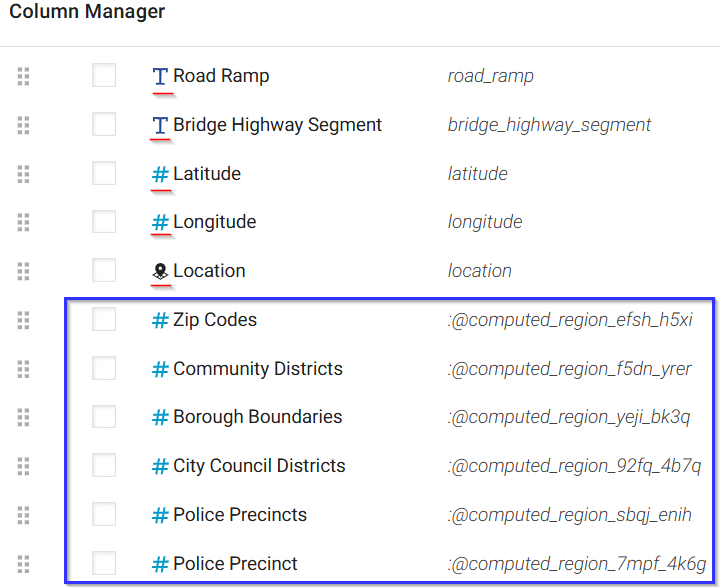
\includegraphics[scale = 0.7]{computed_columns_screenshot.png}
	  \caption{Screenshot of data portal showing the ``@computed'' columns}
	  \label{fig:computed-columns}
\end{figure}

This, of course, raises several questions:
\begin{itemize}
	\item How are these fields computed? Using what source data? Using what computational method?
	\item How can these fields be verified or cross-checked?
	\item Why are their two fields that appear redundant ``Police Precinct'' and ``Police Precincts''?
	\item What are ``borough boundaries''? Are these the regular NYC boroughs?
	\item What are ``community districts''? Is this the same as the ``Community Boards'' that are part of the NYC government?
	\item Can these fields be included in the official 311 SR Data Dictionary?
	\item Can these fields be used for analytical purposes? 
\end{itemize}	

The last bullet point is the key here. Are these fields reliable and accurate, and can they be used for subsequent analysis? Unfortunately,
as of this date, those questions have not been fully addressed by the  NYC Open Data Team. This paper will address further issues with the
accuracy and subsequent analytical usage for these six @computed fields.
	
	
\section{Verifying data types}
Fortunately, both the Data Dictionary and the portal column manager do a good job of indicating the data type.
As indicated by the red underline in Figure \ref{fig:computed-columns}, there is a small icon next to the column name 
which indicates the data type of the column. The stylized capital ``T'' indicates text, the ``\#'' sign indicates 
a numeric, a calendar icon indicates a date field, and the ``pin on a map'' symbol indicates a geospatial field. 
	
The following fields were checked for their specified data types:
	
\begin{itemize}
	\item created\_date, closed\_date, due\_date, and resolution\_action\_updated\_date are all in proper date format.
	\item zip\_codes and incident\_zip: All are 5 numeric digits except for 2 non-numeric entries for incident\_zip (``na'' and ``N/A'').
	\item x\_coordinate\_state\_plane \&  y\_coordinate\_state\_plane (a NY State geo-location system) are all numeric.
	\item latitude \& longitude are both numeric.
	\item community\_districts, borough\_boundaries, city\_council\_district, police\_precinct, and police\_precincts are all numeric.
	\item Free-form text fields that contain a ``,'' (e.g. incident\_address, resolution\_description) are enclosed in quotation marks.
\end{itemize}	
	

\section{Blank \& N/A data}

Understanding the absence of data in each fields is an important factor when undertaking analysis. For example, if you wanted to see if the SRs were
closed before or after their due\_date, you would be challenged as 99.57\% of the due\_date field is blank. (Although with such a large dataset
that still leaves 24,411 values, all of which are N/A, which calls into question are these missing values, or is the specification of a
due\_date simply not applicable for the vast majority of SRs?)

When counting the various fields for blank or N/A values, the dataset appears to divide into three groups: Mostly Empty, Partially Empty, and Few/None Empty.
The Mostly Empty category ranges from 93-99.9\% blank and includes such fields as taxi\_company due\_date, pickup\_location, and landmark. The Partially 
Empty includes such fields as location\_type, borough, and cross\_street. And the Few/None Empty includes created\_date, complaint\_type, agency, and status.
In some cases it may make sense to inquiry as to why some fields are frequently blank. Is the data difficult to capture? Does it pertain to only a small set
of complaint\_type or Agencies? And if the data is truly that sparse, does it make sense to even collect it. For example, you would think that every complaint
that every SR that has a geographical component, such as an address, would also have a corresponding police\_precinct and community\_district since these
are all-inclusive. That it would have a lat/long.  But indeed these fields do have small, but nonetheless significant empty entries. 

During the analysis, it was determined that the following fields are mandatory, and any rows missing these fields is removed from the dataset (which very, very
rarely occurred fortunately): created\_date, agency, complaint\_type, and unique\_key. 

\begin{table}[ht]
\centering
\caption{Blank and N/A entries by field}
\resizebox{0.8\linewidth}{!}{%
\tiny
\begin{tabular}{lrrrl}
	\toprule
	\textbf{Field} & \textbf{Total Empty} & \textbf{Percent Empty} & \textbf{N/A Count} \\
	\midrule
		taxi\_company\_borough & 6391341 & 99.94 & 0 \\
		road\_ramp & 6379080 & 99.75 & 0 \\
		vehicle\_type & 6376266 & 99.71 & 0 \\
		due\_date & 6370497 & 99.62 & 6370497 \\
		bridge\_highway\_direction & 6367626 & 99.57 & 0 \\
		bridge\_highway\_name & 6340197 & 99.14 & 0 \\
		bridge\_highway\_segment & 6340190 & 99.14 & 0 \\
		taxi\_pick\_up\_location & 6329954 & 98.98 & 0 \\
		facility\_type & 5966588 & 93.30 & 0 \\
		landmark & 2635736 & 41.22 & 0 \\
		intersection\_street\_1 & 2143847 & 33.52 & 0 \\
		intersection\_street\_2 & 2140707 & 33.48 & 0 \\
		cross\_street\_1 & 1846594 & 28.88 & 0 \\
		cross\_street\_2 & 1846008 & 28.87 & 0 \\
		location\_type & 798775 & 12.49 & 0 \\
		bbl & 768109 & 12.01 & 0 \\
		city & 332086 & 5.19 & 0 \\
		street\_name & 280463 & 4.39 & 0 \\
		incident\_address & 280268 & 4.38 & 0 \\
		closed\_date & 248839 & 3.89 & 248839 \\
		resolution\_description & 132333 & 2.07 & 0 \\
		zip\_codes & 123167 & 1.93 & 0 \\
		borough\_boundaries & 101453 & 1.59 & 0 \\
		community\_districts & 101445 & 1.59 & 0 \\
		city\_council\_districts & 101445 & 1.59 & 0 \\
		police\_precincts & 101445 & 1.59 & 0 \\
		police\_precinct & 101416 & 1.59 & 0 \\
		latitude & 99778 & 1.56 & 0 \\
		longitude & 99778 & 1.56 & 0 \\
		location & 99778 & 1.56 & 0 \\
		x\_coordinate\_state\_plane & 99668 & 1.56 & 0 \\
		y\_coordinate\_state\_plane & 98822 & 1.55 & 0 \\
		resolution\_action\_updated\_date & 91399 & 1.43 & 91399 \\
		incident\_zip & 83220 & 1.30 & 2 \\
		descriptor & 74645 & 1.17 & 0 \\
		address\_type & 38655 & 0.60 & 0 \\
		unique\_key & 0 & 0.00 & 0 \\
		agency & 0 & 0.00 & 0 \\
		agency\_name & 0 & 0.00 & 0 \\
		complaint\_type & 0 & 0.00 & 0 \\
		status & 0 & 0.00 & 0 \\
		community\_board & 0 & 0.00 & 0 \\
		borough & 0 & 0.00 & 0 \\
		open\_data\_channel\_type & 0 & 0.00 & 0 \\
		park\_facility\_name & 0 & 0.00 & 0 \\
		park\_borough & 0 & 0.00 & 0 \\
		created\_date & 0 & 0.00 & 0 \\
	\bottomrule
\end{tabular}
}
\end{table}

\FloatBarrier % Ensure all floats before this point are processed before moving on

Here is a graphic depiction of total empty (blank \& N/As) for each fields. You can see the natural grouping into the Most, Some, and Few categories. 

\begin{figure}[H]
  \centering
	  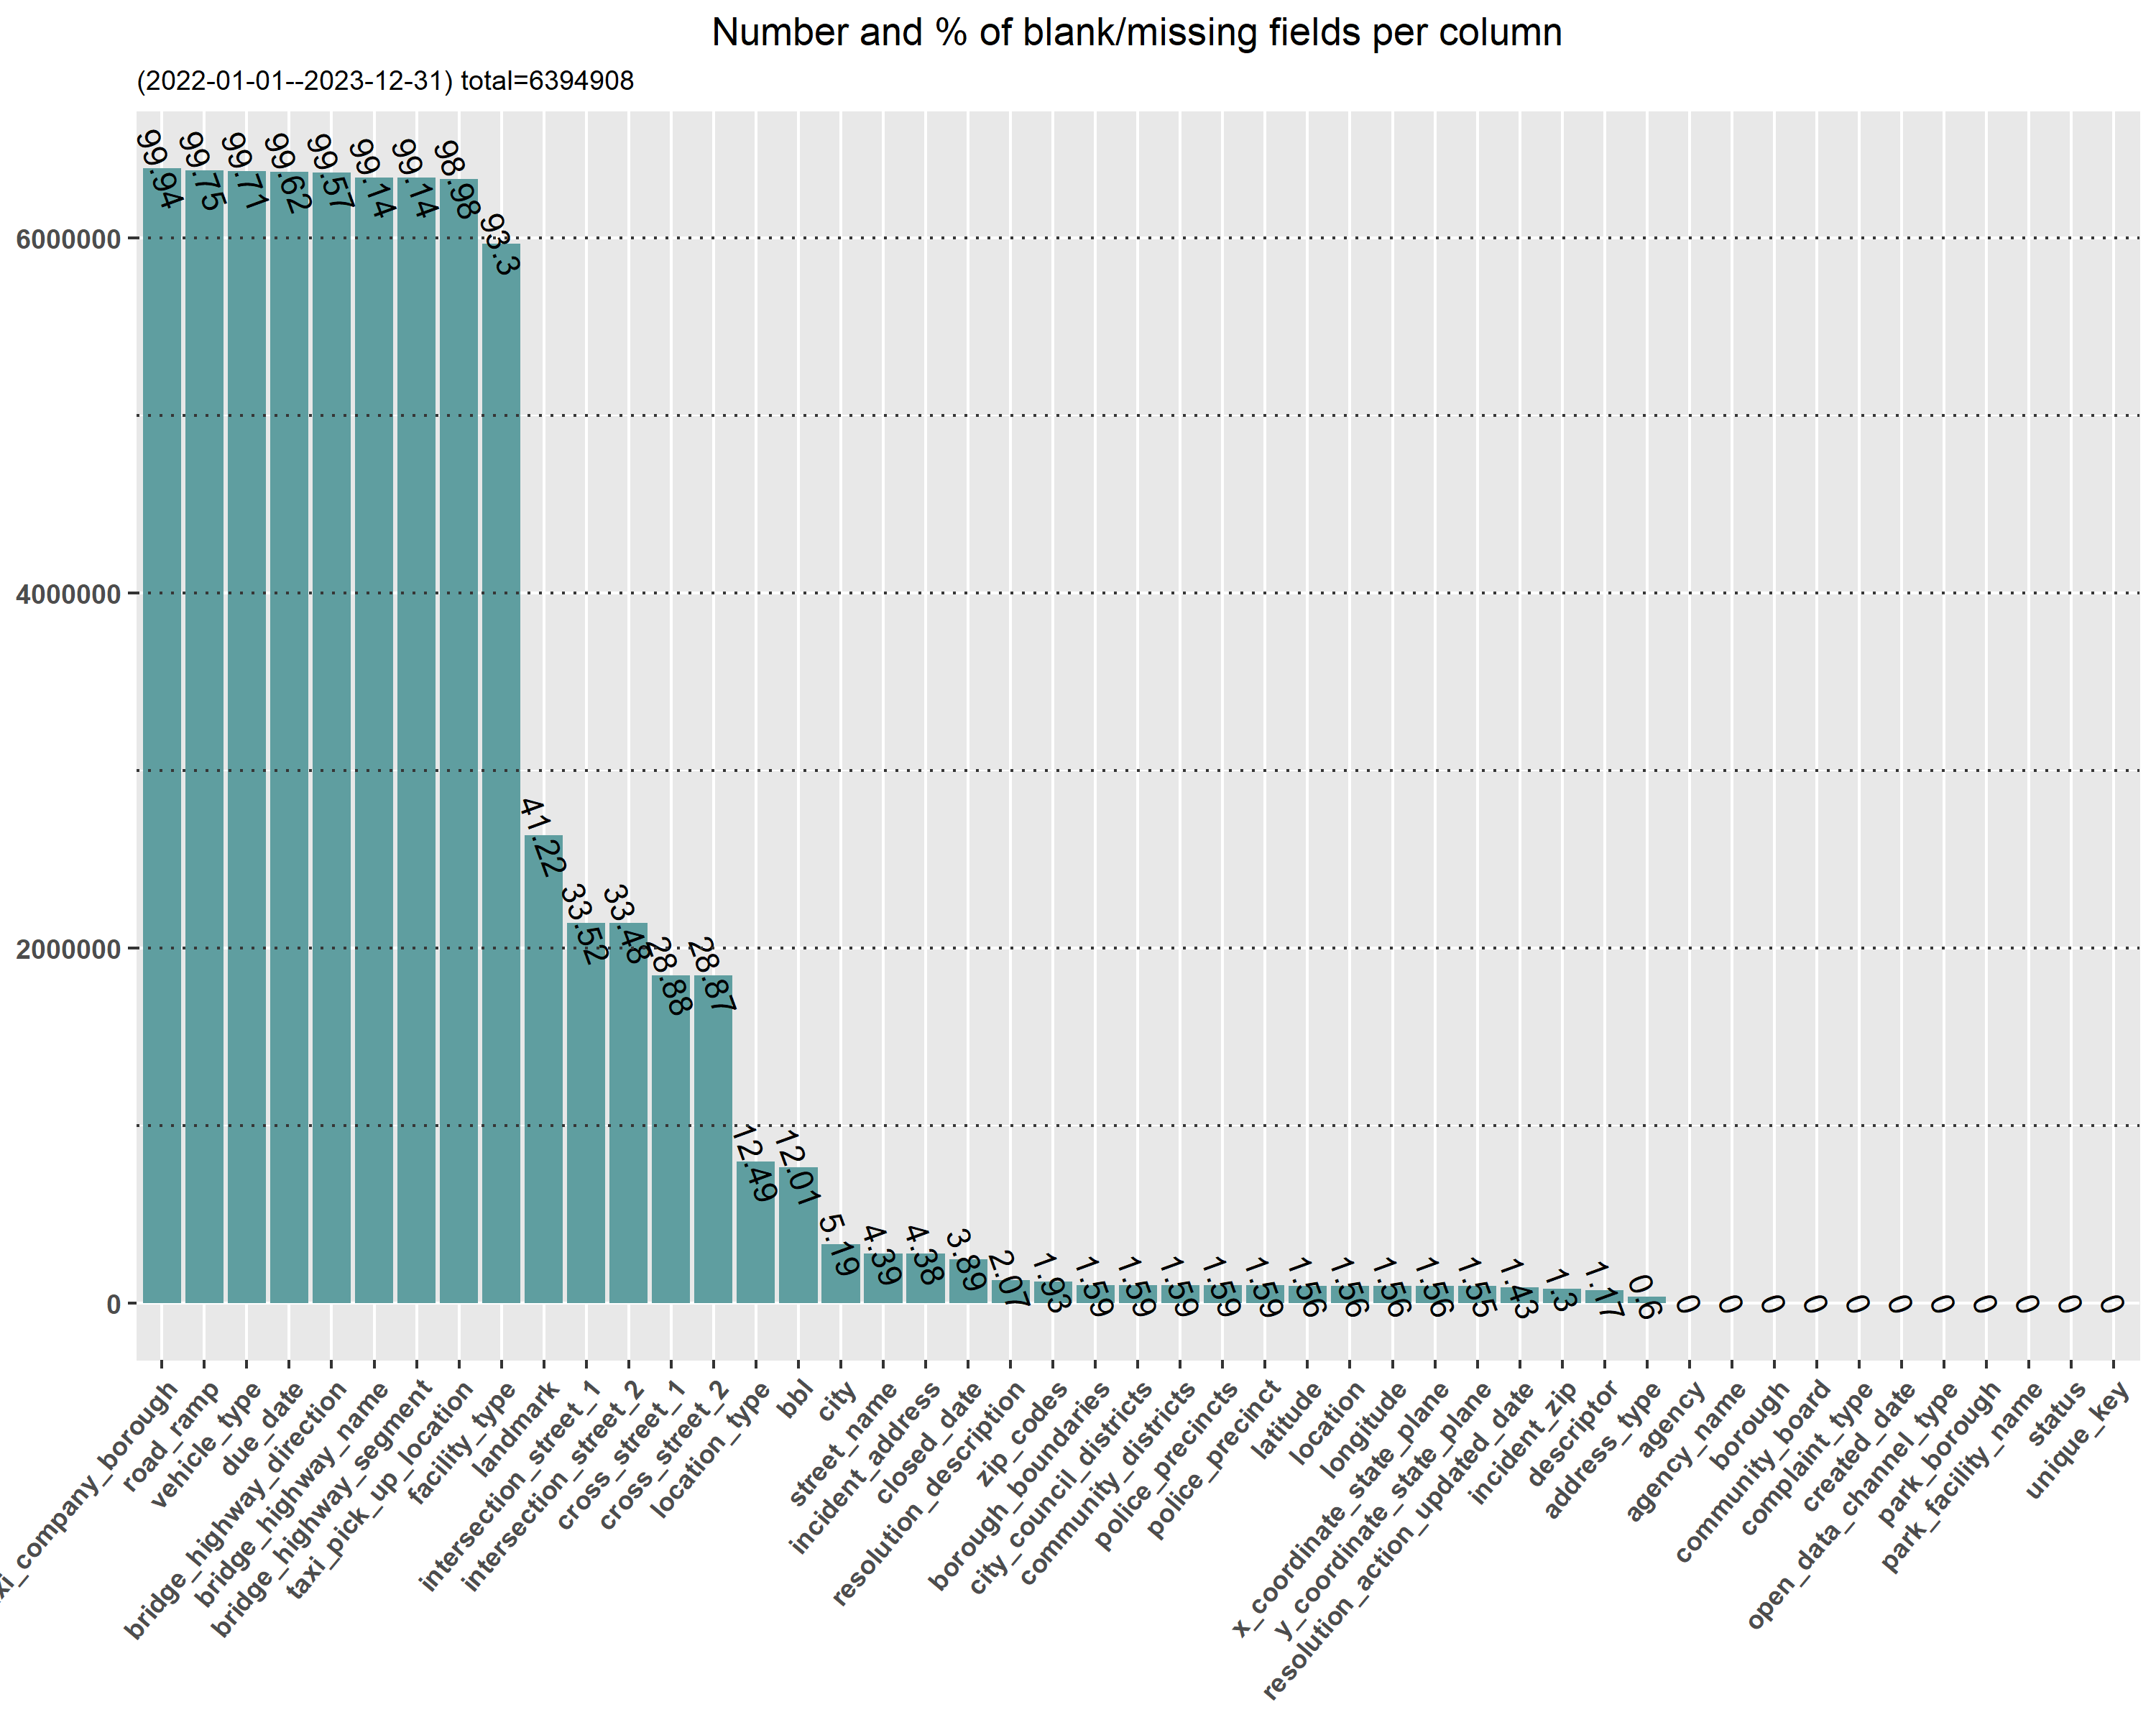
\includegraphics[width=\textwidth]{BlankFields.png}
	  \caption{Number and Percentage of Empty Entries}
	  \label{fig:blank_fields}
\end{figure}


\section{Data type correctness}

All data fields were subjected to a test of ``correctness'' according to their ``type'' as specified
in the Data Dictionary.  Of the nearly 300 million data fields to check (6.5 million rows, 47 fields per row), there were only two  values that failed to test for the
proper data type; those being two text entries in the incident\_zip filed (``na'', and N/A). All date fields were dates. All number fields were numeric. All text
fields were character.

 
 \section{Validating data}
 While the dataset may have fields populated with data that appears correct, it is necessary to inspect those fields to determine if the data is indeed valid. For
 example a date field that contains the value ``February 30, 2024'' is clearly not valid. Nor is a latitude of +95 deg north. 
 
 In this study, testing for invalid values revealed several serious issues associated with select fields. Accordingly, an analyst would need to be
extra diligent if using these fields for analysis. In all likelihood, rows with invalid field values would likely need to be removed from the
analysis dataset.

Some fields can be validated against either a acceptable values, often drawn from historical context. In this study we looked at a 10-year
dataset to ascertain a domain for values what do not have a specific reference source. We would recommend that these domains be published
in the Data Dictionary. Here are some results.

\begin{itemize}
	\item Latitude and Longitude fields were tested to ensure all fell within the geographic boundaries of the City of New York. All were.
	\item The unique\_key field was in fact unique.
	\item Many fields have a domain of acceptable values. Often these values are determined from common usage or by examining
	larger historical datasets. Unfortunately, these domains of acceptable values are not specified in the Data Dictionary. These fields all tested as
	compliant with their domain of acceptable values:
		\begin{itemize}
			\item address\_type
			\item status
			\item borough, borough\_boundaries, \& park\_borough 
			\item data\_channel
			\item vehicle\_type
			\item city\_council\_district
		\end{itemize}
\end{itemize}	

	\subsection{Issues with Zip Codes}
	 Unfortunately some fields did prove to be quite problematic when comparing the values to the domain of legal values.
	 For example, all zip codes (two fields: zip\_codes and incident\_zip) should be valid as defined by the USPS database
	 which contains over 44,000 valid zip codes.
	 
	The computed field zip\_codes proved especially problematic with 58\% (3.6 million) of the field entries being invalid.
	This high number indicates that the computation of this computed fields is highly inaccurate. We would recommend
	dropping this field for future analytic efforts.
	
	Furthermore, the field incident\_zip while having only .07\% invalid entries, that is still 4163 such errors. As zip code is
	a primary measure of many NYC city services, and with a freely available database for which to validate entries
	against, it seems an oversight that any such errors could creep into the system. Some invalid entries are 
	clearly incorrect just by observation, e.g. 10000, 12345, 11111, etc. 
	
	Because zip codes play a significant role in analyzing City services, these errors can be quite serious. It's useful in 
	such cases to observe the breakdown of these errors by the responsible Agency. 
	
	The breakdown of the invalid entries in the zip\_code, sorted by Agency shows that the distribution by percentage
	almost precisely mirrors the overall breakdown of SRs by Agency. This indicates a systemic problem, and since the
	zip\_code fields is one of the computed fields, it appears these errors are caused by incorrect computations rather
	than by any Agency mistake.
	
	The  errors in the incident\_zip field are more troubling, even though they are, percentage-wise, small. Here is a graphic 
	illustrating how these errors occur by Agency. Here we can see that the majority of these errors lie in the Dept of Transportation,
	NYPD, Taxi \& Limo Commission (TLC), and the Economic Development Council (EDC) among others. This representation
	does not follow the full SR distribution indicating that these errors are likely generated by an incorrect
	process or application residing at those particular Agencies; it is not a systemic problem.

	\begin{figure}[H]
	  \centering
		  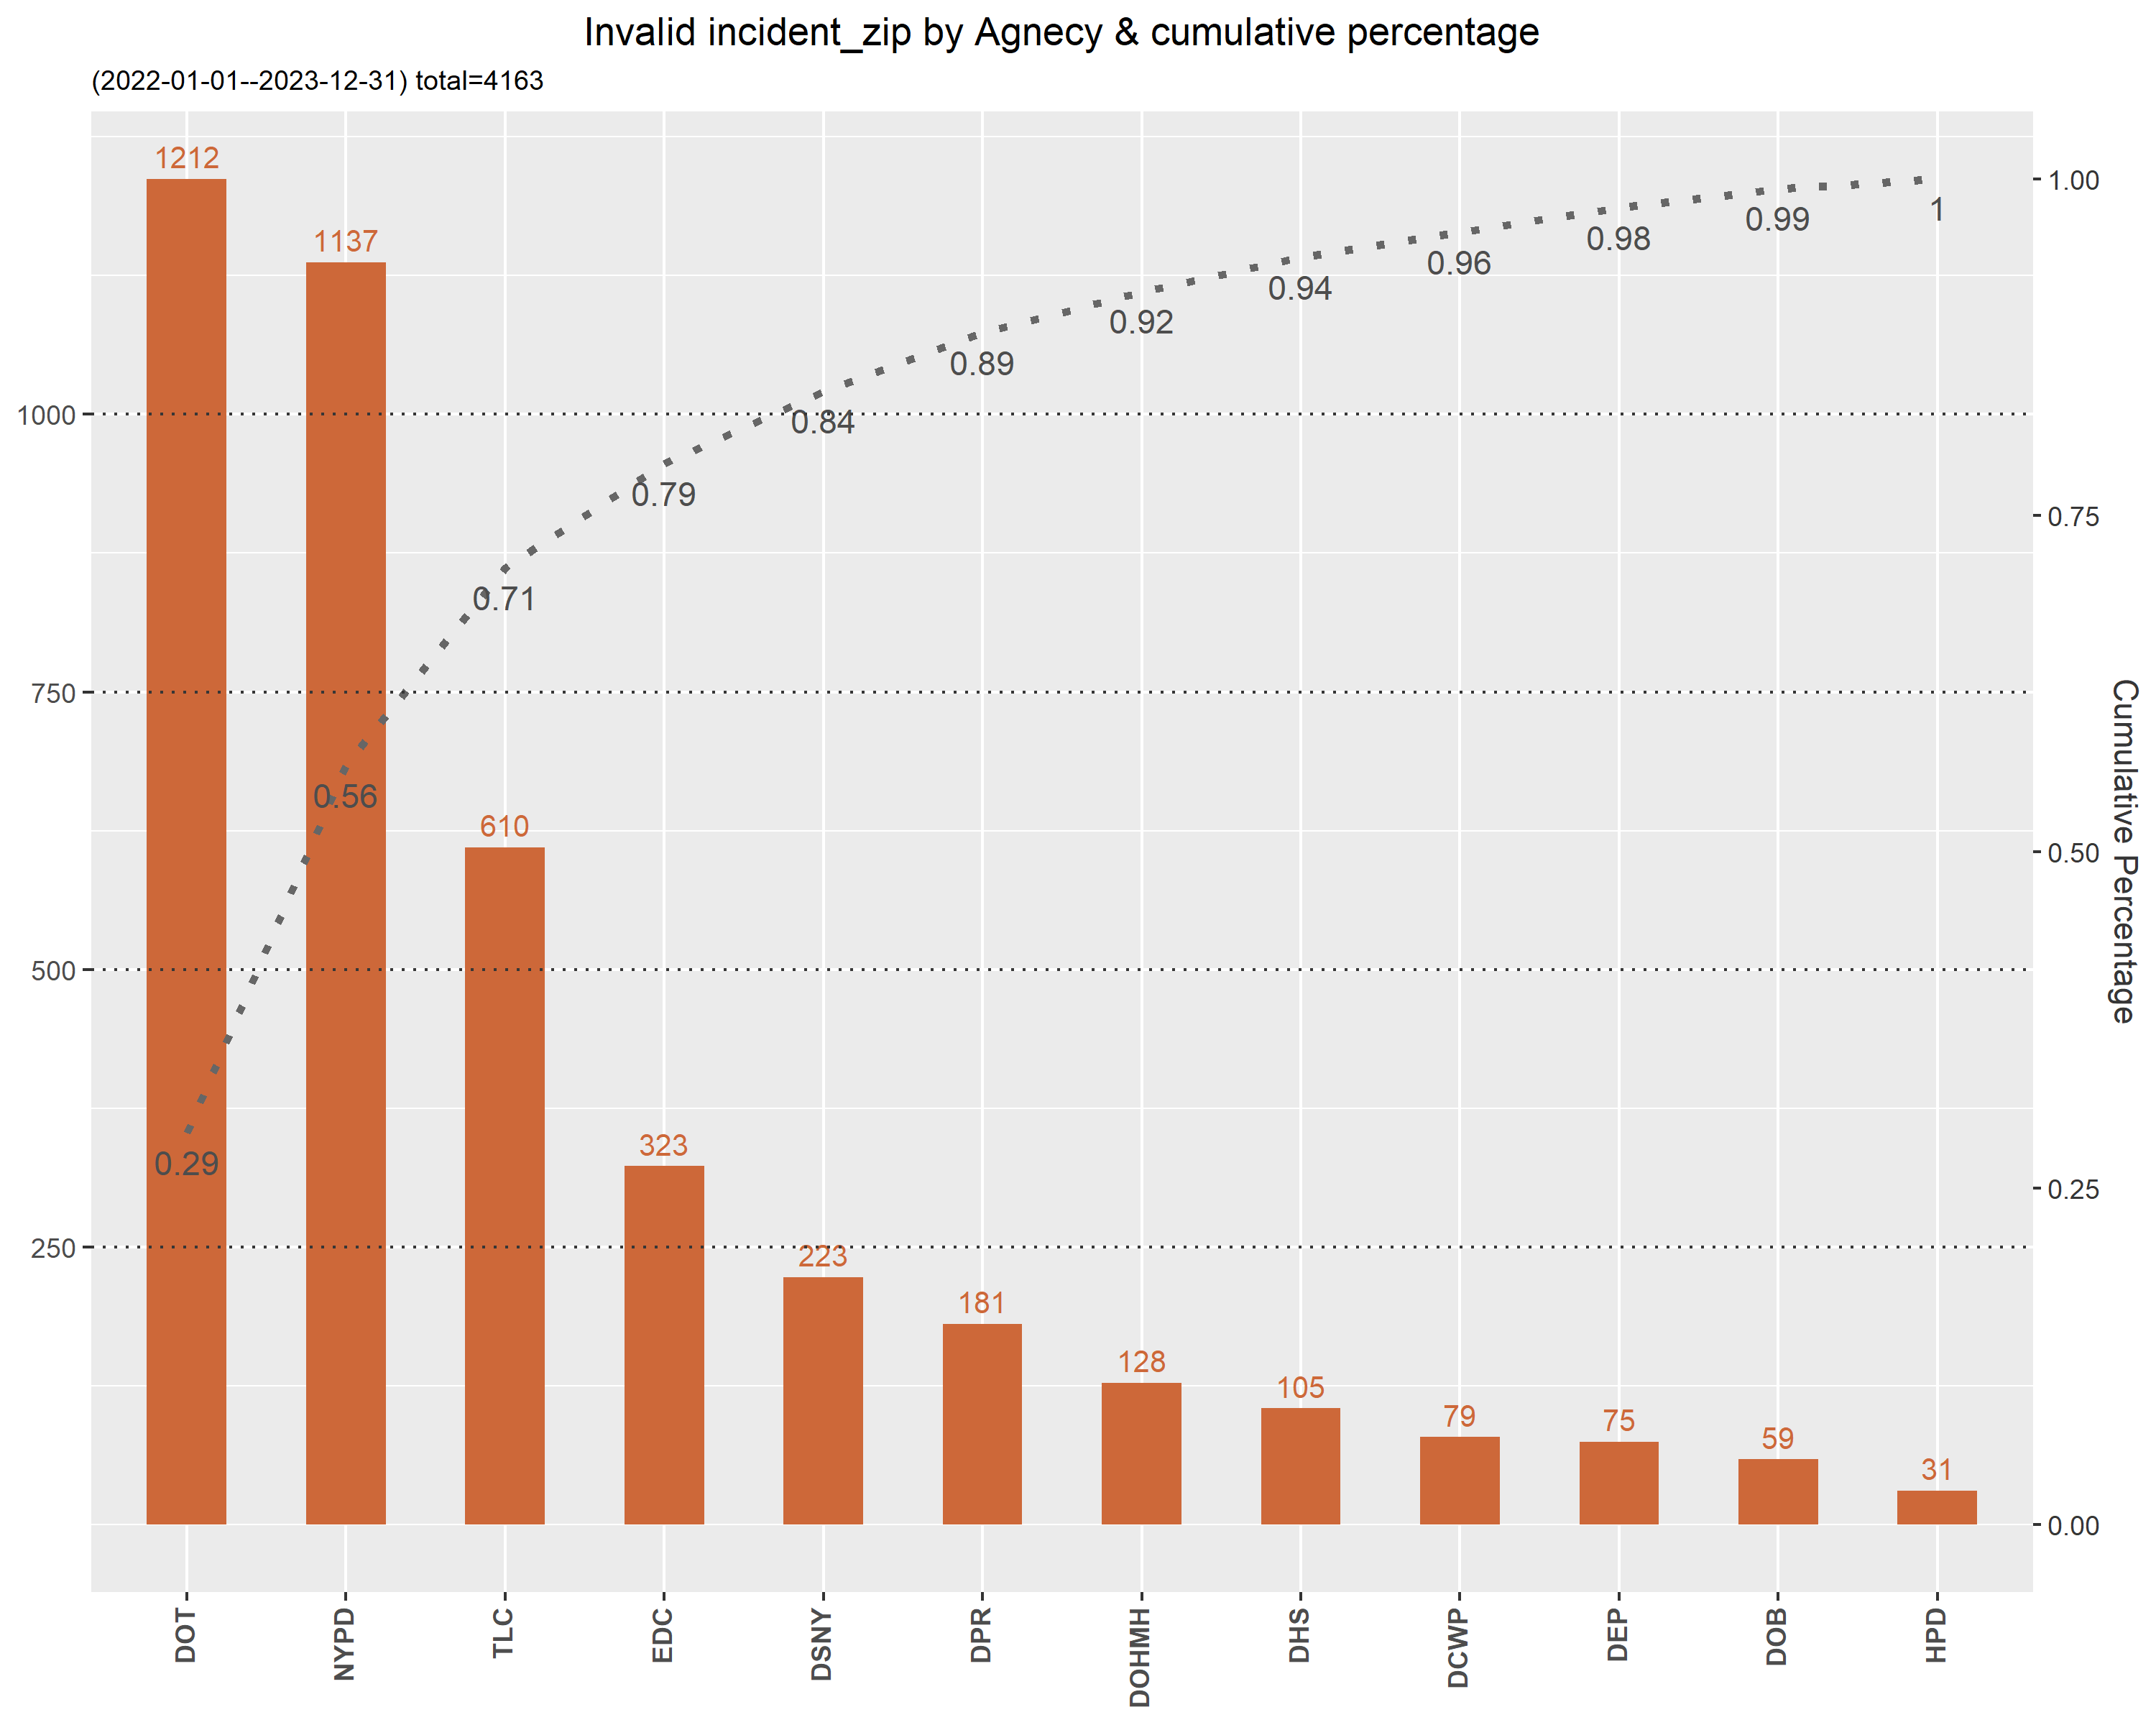
\includegraphics[width=\textwidth]{invalid_incident_zip.png}
		  \caption{Invalid incident-zip by Agency}
		  \label{fig:invalid_incident_zip}
	\end{figure}
	
		\subsubsection{Case Study: Noise Complaints by Zip Code}
		\textbf{Scenario:} The NYC Office of Nightlife (ONL) wants to know ``What are the top 10 zip codes for Noise Complaints (all 8 types) over the last two years?''
		The goal is to assess the impact of the recent NYC effort looking to promote a safe and vibrant nightlife scene in NYC while seeking to ease
		strained relations between bar and club owners. 
		
		It may come as a surprise to non-NYC residents that dancing at bars and restaurants has been illegal since 1926 (during prohibition), and was only just repealed in 2018. 
		
		On the surface this would seem like a simple effort.  The NYC Open Data Portal allows for selection of a timeframe (2022-2023), complaint-type
		begins with ``Noise'', and group by Zip code, sorted descending by count.  You can do this analysis and grouping right inside the NYC Open Data Portal. \textit{Voila!}

	\begin{figure}[H]
	    		\centering
	    		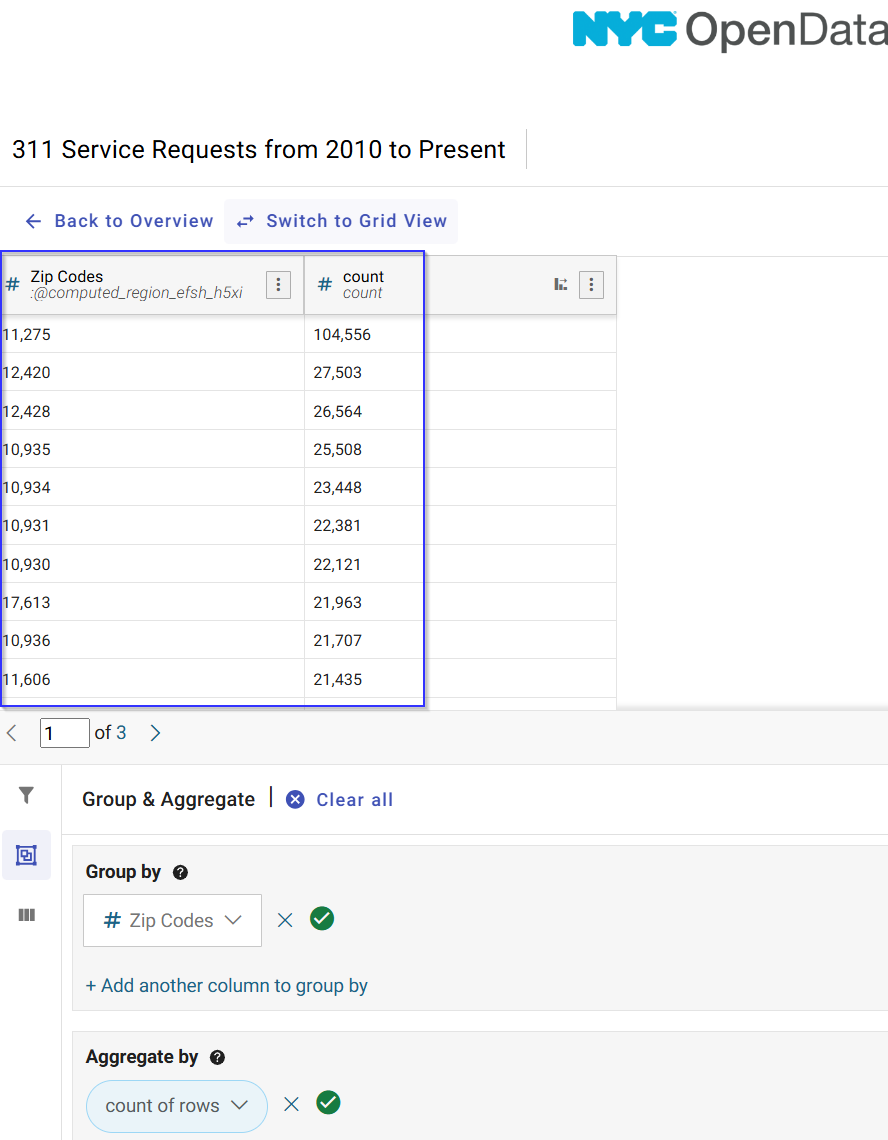
\includegraphics[scale = 0.6]{zipcode_casestudy.png}
	    		\caption{Top 10 zip codes for Noise complaints (Zip Codes)}
	    	\label{fig:casestudy1-zipcodes}
		\end{figure}
	
		However, this analysis uses the zip\_codes field, one of the (six) computed fields that has shown to have validity problems. If we repeat the analysis with the 
		incident\_zip field instead of the zip\_codes field, we obtain a different set of zip code results:
		
		\begin{figure}[H]
	    		\centering
	    		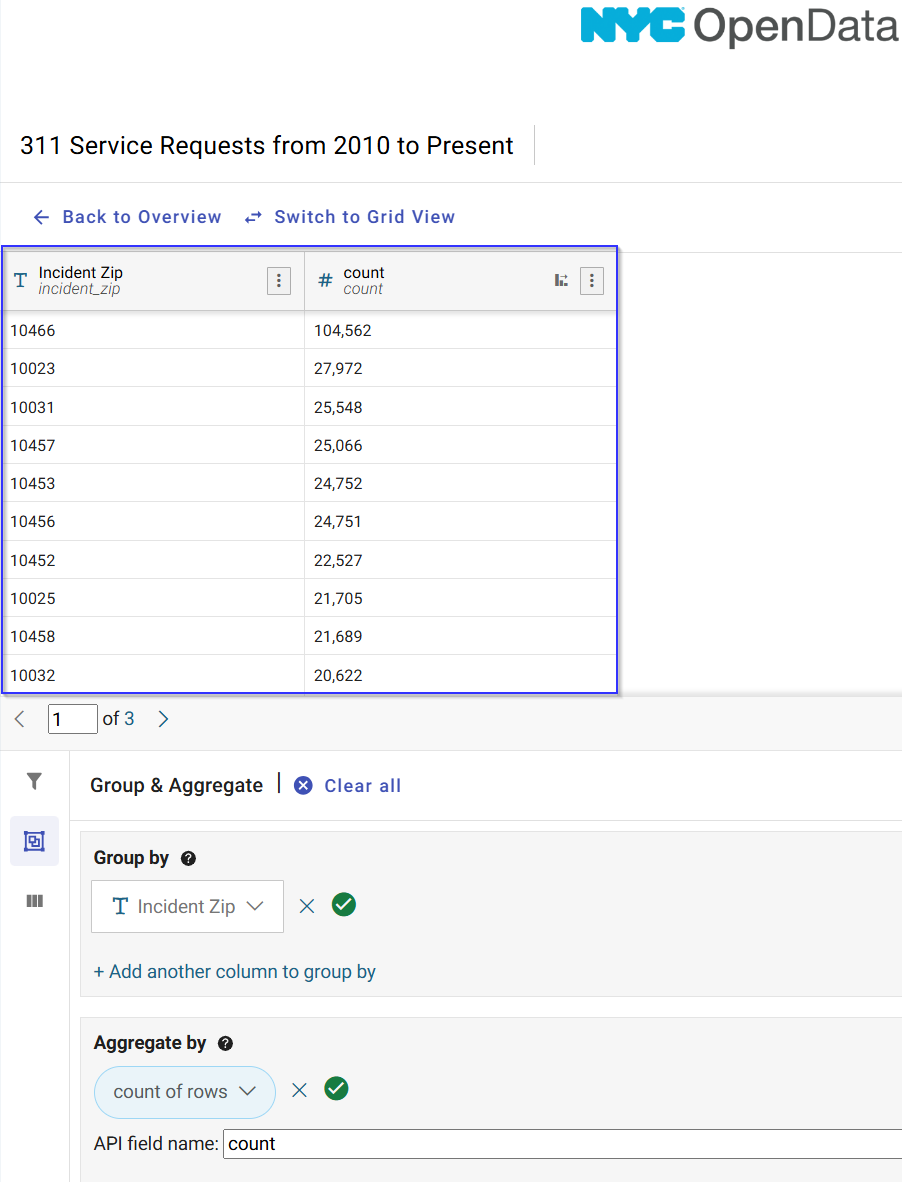
\includegraphics[scale = 0.6]{incident_zip_casestudy.png}
	    		\caption{Top 10 zip codes for Noise complaints(Incident Zip)}
	    	\label{fig:casestudy1-incident-zip}
		\end{figure}
		
	Let's subject these two data sets to validation against the US Postal Service zip code database.
	 
	\begin{table}[H]
	\centering
	\footnotesize
	\caption{Comparison of Top Ten Zip Codes Lists}
	\begin{tabular}{lrr@{\hskip 0.5cm}|@{\hskip 0.5cm}lrr}
	\toprule
	\multicolumn{3}{c}{\textbf{zip\_codes}} & \multicolumn{3}{c}{\textbf{incident\_zip}} \\
	\cmidrule(r){1-3} \cmidrule(l){4-6}
	\textbf{Zip Code} & \textbf{Count} & \textbf{Valid?} & \textbf{Zip Code} & \textbf{Count} & \textbf{Valid?} \\
		\midrule
		11275 & 104,556 & FALSE & 10466 & 104,562 & TRUE \\
		12420 & 27,503 & TRUE & 10023 & 27,972 & TRUE \\
		12428 & 26,564 & TRUE & 10031 & 25,548 & TRUE \\
		10935 & 25,508 & FALSE & 10457 & 25,066 & TRUE \\
		10934 & 23,448 & FALSE & 10453 & 24,752 & TRUE \\
		10931 & 22,381 & TRUE & 10456 & 24,751 & TRUE \\
		10930 & 22,121 & TRUE & 10452 & 22,527 & TRUE \\
		17613 & 21,963 & FALSE & 10025 & 21,705 & TRUE \\
		10936 & 21,707 & FALSE & 10458 & 21,689 & TRUE \\
		11606 & 21,435 & FALSE & 10032 & 20,622 & TRUE \\
		\bottomrule
	\end{tabular}
	\end{table}

	As indicated, six out of ten zip\_codes are invalid, which corresponds closely with what is observed in the overall dataset (58\%). Whereas the incident\_zip
	field is completely valid, again in-line with the overall incident\_zip validation percentage (99.04\%)
	Perhaps more curious than the differing zip codes on the two lists, is the fact that the numerical counts are nearly identical;  the overall counts are quite close. This is curious since
	one field is computed while the other is via data entry; the computed protocol is again the suspect.

	
	\subsection{Issues with Police Precincts}
	A curious case also exists when examining the two nearly identical fields - police\_precincts and police\_precinct. Both of those fields are among
	the ``computed'' fields in the dataset. 
	Using  \href{https://www.nyc.gov/site/nypd/bureaus/patrol/precincts-landing.page}{NYPD Precinct listings} it's possible to determine the valid
	police precincts; they are generally numeric or have numeric representations in the dataset. 
	
	However, what we find is that both fields police\_precinct and police\_precincts  have  35\% invalid entries.
	Unfortunately, they're not the same invalid entries. 
	
	For the police\_precincts field, there are 2,171,864 invalid entries (35\%)., a consequential number of errors. Similarly for the police\_precinct field,
	 there are 2,171,778 invalid entries ( also 35\%), however they are not the same counts for the two similar fields.

	The top ten (by count) of invalid precincts are:

	\begin{table}[ht]
	\footnotesize
	\centering
		\begin{tabular}{ccccc}
		\toprule
		\textbf{Invalid Precinct} & \textbf{police\_precinct count} & \textbf{police\_precincts count} & \textbf{Delta}\\
		\midrule
			62 & 151808 & 151720 & 88 \\
			72 & 148881 & 148796 & 85 \\
			67 & 133171 & 133115 & 56 \\
			64 & 111236 & 111221 & 15 \\
			60 & 105252 & 105317 & -65 \\
			65 & 103334 & 103306 & 28 \\
			53 & 100097 & 100074 & 23 \\
			73 & 97746 & 97755 & -9 \\
			68 & 94204 & 94254 & -50 \\
			66 & 93654 & 93848 & -194 \\
		\bottomrule
		\end{tabular}
	\caption{Comparison of the fields police\_precinct and police\_precincts}
	\label{tab:comparison-precincts-diff}
	\end{table}
	
	A graphic representation of the invalid police\_precincts plotted by Agency show a near perfect match to the
	distribution of the entire 6.4 million SRs. Note that the ``big six'' Agencies account for 90\% of these invalid precinct errors, identical
	to the overall distribution of all SRs. This strongly suggests that this is a systemic problem, almost certainly
	caused by the computation method applied for these two fields.
	 
	\begin{figure}[H]
	  \centering
		  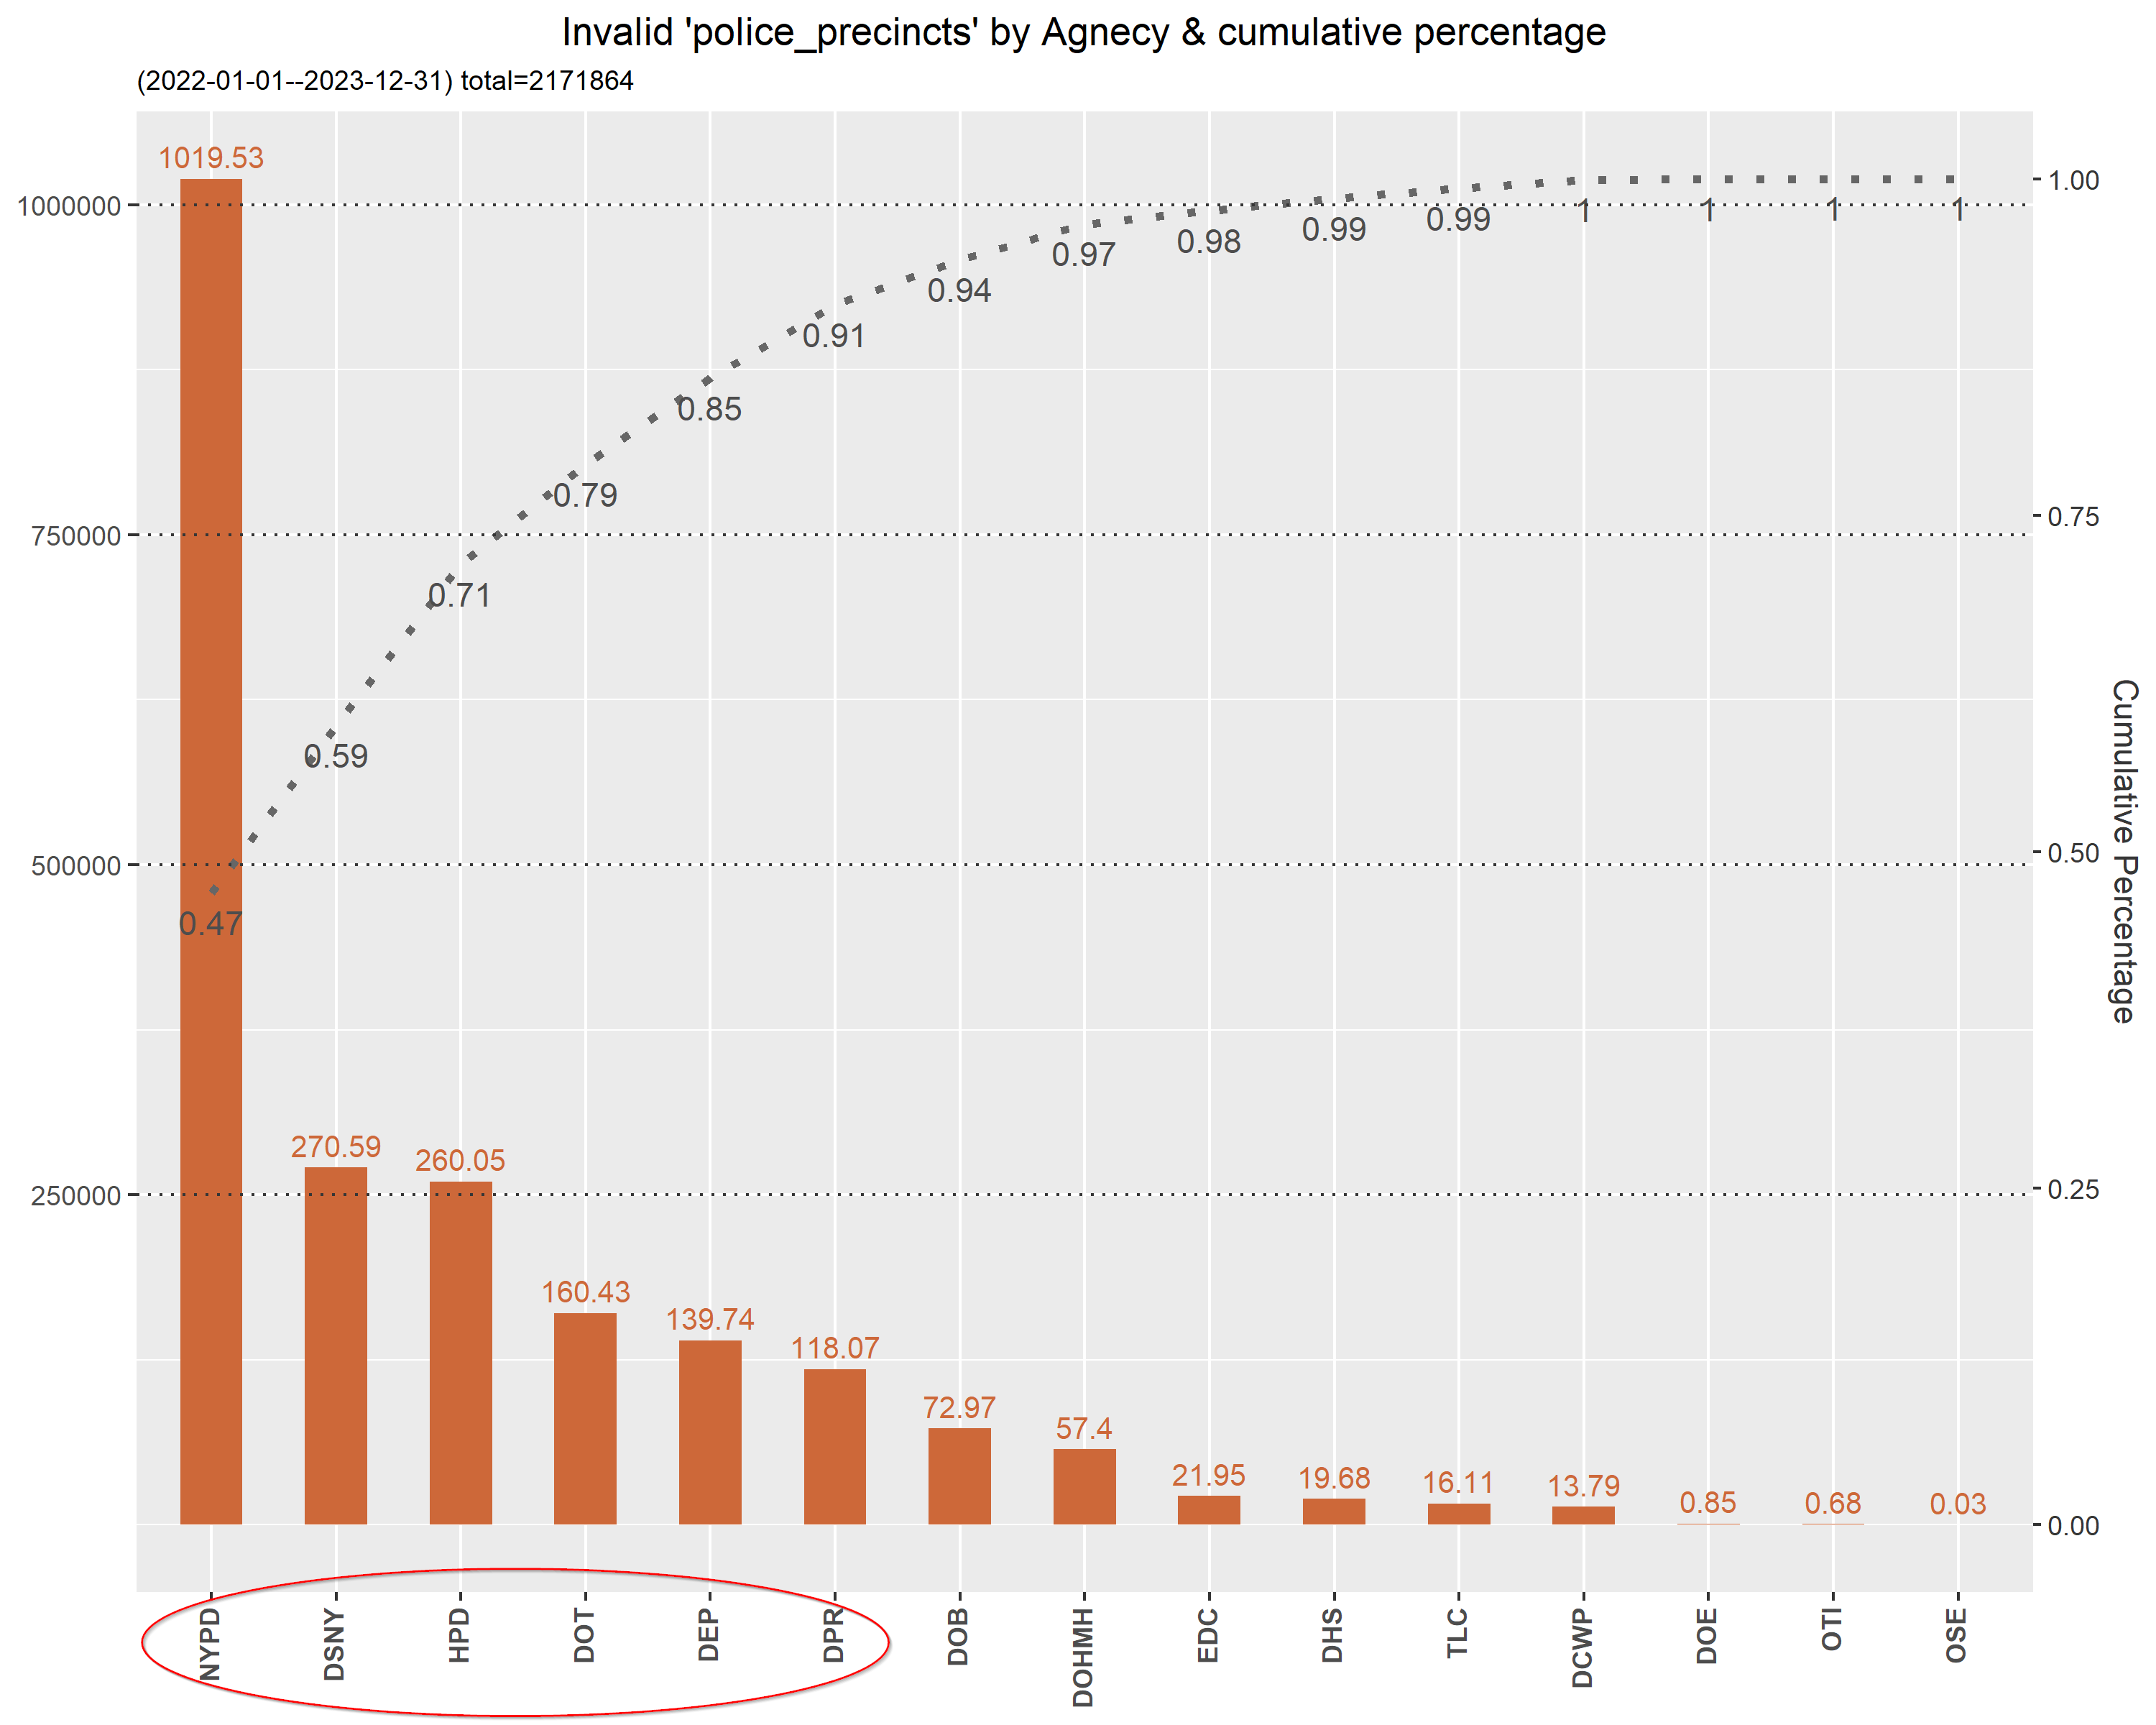
\includegraphics[width=\textwidth]{invalid_police_precincts.png}
		  \caption{Invalid NYPD precincts by Agency}
		  \label{fig:invalid_police_precincts_zip}
	\end{figure}

	\subsection{Issues with Community Boards}
	Community Boards are an important aspect of NYC government. Community boards are the most local, grassroots form of City government, 
	and the connection between communities and elected officials and City agencies. They are organized by the five Boroughs of NYC and represented
	in this dataset as ``\#\#-Borough'', e.g. ``10 Bronx''. As such, they play an important role in the quality of life for all New Yorkers. There are 59 community boards 
	throughout the City. There are 12 Community Districts in the Bronx, 18 in Brooklyn, 12 in Manhattan, 14 in Queens and 3 in Staten Island. The Community Boards are
	used frequently as a way to measure City services throughout the five boroughs, so correctness is important. NYC Borough Presidents in particular are focused
	on the services offered at the Community Board level.
	
	In the 2022-2023 dataset there are 27,276 invalid community\_board entries which represents 0.43\% of non-blank data. There are a total of 12 different invalid community boards.
	These include: 
	
		\begin{table}[H]
		\centering
		\small
		\caption{Top Ten Invalid 'community\_board' Values}
		\begin{tabular}{rlr}
		\toprule
		\textbf{Rank} & \textbf{Invalid CB} & \textbf{Count} \\
			\midrule
				1 & 64 MANHATTAN & 7144 \\
				2 & 83 QUEENS & 5133 \\
				3 & 55 BROOKLYN & 3327 \\
				4 & 81 QUEENS & 3180 \\
				5 & 80 QUEENS & 2407 \\
				6 & 26 BRONX & 2364 \\
				7 & 28 BRONX & 1128 \\
				8 & 82 QUEENS & 1054 \\
				9 & 95 STATEN ISLAND & 515 \\
				10 & 27 BRONX & 514 \\
			\bottomrule
		\end{tabular}
		\end{table}
		
		The distribution of invalid Community Boards by Agency is not consistent with the overall SR Agency distribution. This indicates that there are likely
		specific issues at some key Agencies, in this case Taxi \& Limo Commission (TLC), Parks \& Recreation, etc. It's not a large error, but the division of services
		(and complaints) by Community Board is a well-tracked measure.

		\begin{figure}[H]
	  \centering
		  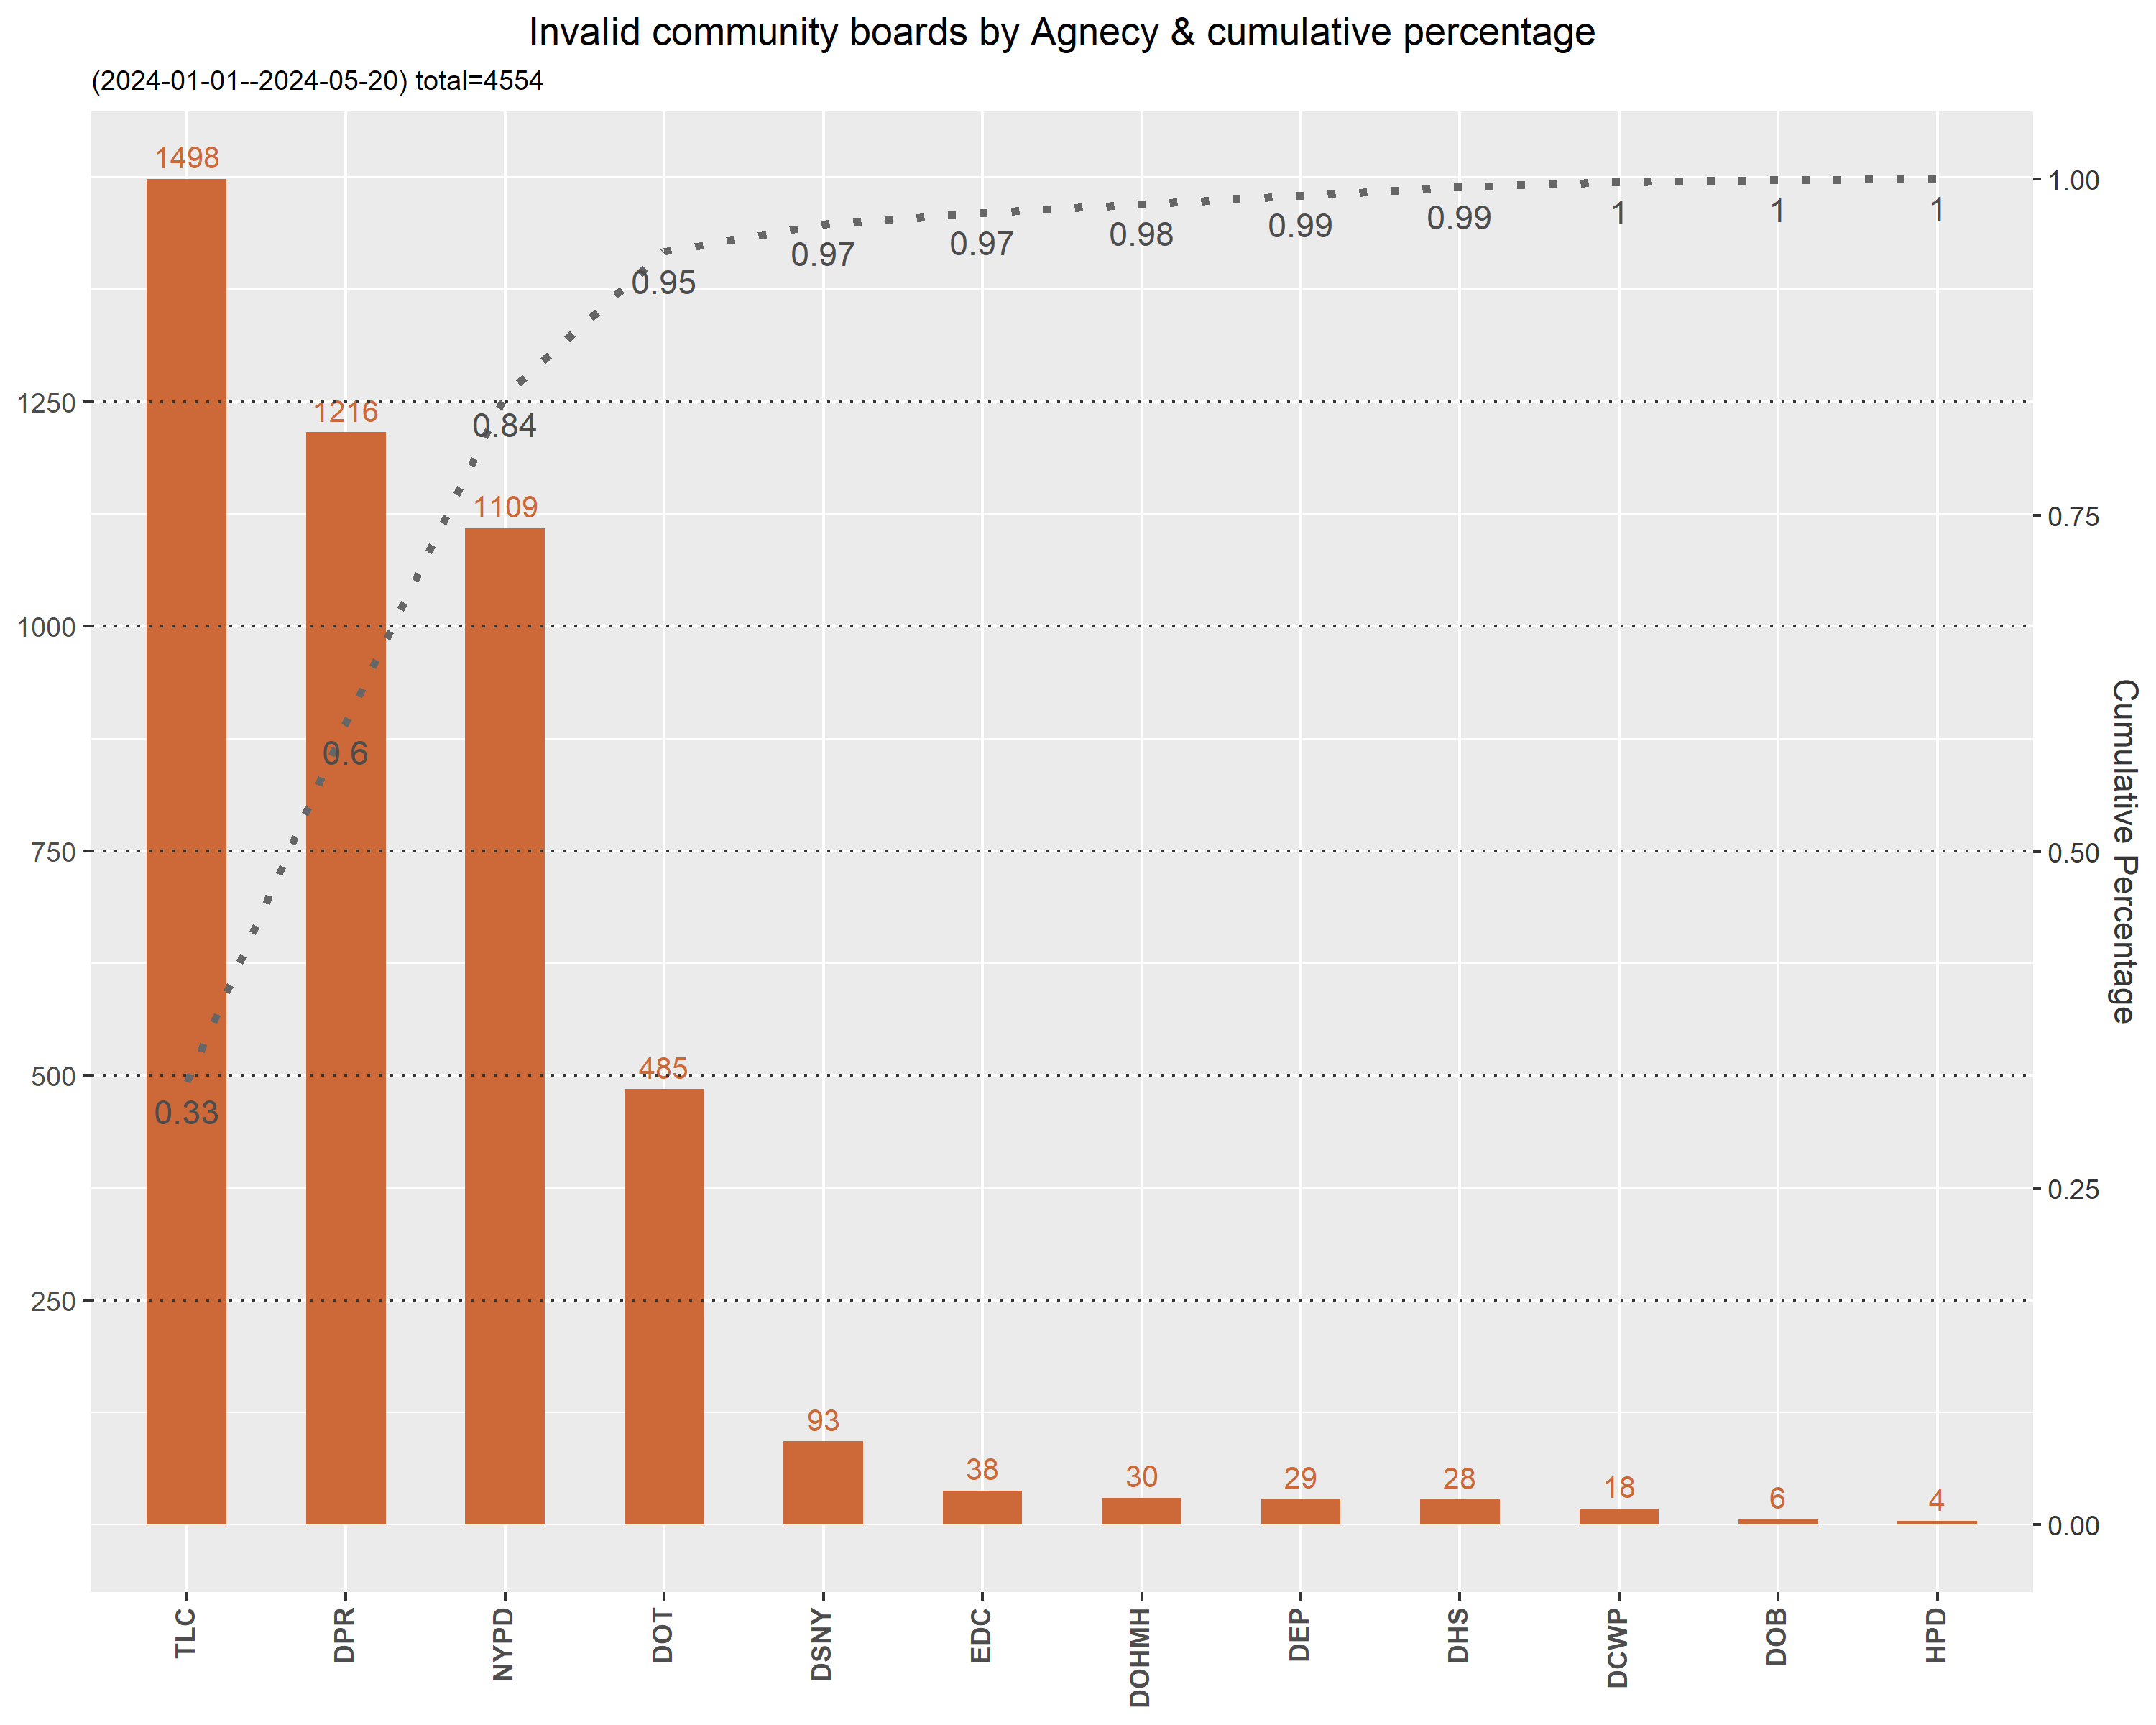
\includegraphics[scale = 0.65]{invalid_community_boards.png}
		  \caption{Invalid Community Board by Agency}
		  \label{fig:invalid_community_boards}
	\end{figure}


	\subsection{Issues with Community Districts}
	Another of the computed fields is community\_districts. Community Districts are the boundaries for the Community Boards, but unlike how Community Boards are
	an arm of the government of New York City, the Community District is used by the Department of City Planning (DCP) for purposes of environmental, socio-economic, and
	demographic purposes. DCP is the NYC''s primary land use agency and is instrumental in the City's physical framework.  It is a geographical division rather
	than a local government division. And like Community Boards, the Community Districts are a frequently used means to breakdown zoning, housing, community facilities,
	and waterfront/open/public spaces. It is also a well-tracked measure.

	Due to how the community\_district data is formatted, it is not possible to establish validity. However, it is possible to determine that the dataset contains
	72 unique entries, while there are only 59 valid Community Districts.
	
\section{Logical inconsistencies }

closed before created (negative duration)
closed exactly as created (zero duration)
closed in the future

\subsubsection Case Study: Homeless Person Assistance

due\_date before created
long resolution\_action\_updated\_date




\section{Accuracy and precision}
There is one area in particular where the question of precision vs. accuracy immediately arises, and that is with the Latitude and Longitude fields.  Both the 
Longitude and Latitude fields are expresses as a 14-decimal number, e.g. 40.86769186022511 (also the Location field which is a straight concatenation of
latitude and longitude). Given that 1 degree of latitude at the equator is equal to 111.044736 kilometers, the ``1'' at the end of that number represents
approximate 1.1104 nanometer or 1/1,000,000,000 of a meter. A DNA molecule is approximately 2nm in width. 

Clearly the representation of the Latitude and Longitude fields are a classic case of 14-digit precision, 
but limited accuracy. It is more likely that the Lat/Long values are accurate to the 5\textsuperscript{th} decimal place, about 3.64 feet; even that might be
overstating things. 

\subsection{Case Study I - Response to Requests for Homeless Person Assistance}

\section{Redundant \& Duplicate data}
Shrinking file size by deleting these 11 redundant fields:
     1 - agency\_name 
     2 - park\_borough 
     3 - borough\_boundaries 
     4 - location 
     5 - intersection\_street\_1 
     6 - intersection\_street\_2 
     7 - police\_precinct 
     8 - duration 
     9 - postClosedUpdateDuration 
     10 - translated\_borough\_boundaries 
     11 - zip\_codes 
Original size: 3.2 Gb 
Size after removing redundant columns: 2.8 Gb 
Potential size reduction: 395.3 Mb or 12.3

\section{Improvements} \label{sec:improve}

Data validation: identify invalid data

Data cleaning: convert to all lower/upper cases;

Data organization: put zipcode/borough in a separate table; verify intersection
== cross; remove redundant columns (and compare how much space saved)

\section{Protocol Suggestions} \label{sec:protocol}

\section{Discussion} \label{sec:disc}


\bibliographystyle{asa}
\bibliography{ref}

\end{document}




\end{document}
